% Self-Certified Continual Learning (SCCL) — Paper (v3)
% Numbers are generated by gcl/report.py from runs/*/metrics.json — never hand-typed.
\documentclass[10pt,conference]{IEEEtran}
\usepackage{amsmath,amssymb,amsfonts}
\usepackage{graphicx}
\usepackage{booktabs}
\usepackage{hyperref}
\usepackage{listings}
\usepackage{xcolor}

\lstset{basicstyle=\ttfamily\footnotesize, breaklines=true, frame=single,
  keywordstyle=\color{blue}, commentstyle=\color{gray}}

% results registry (generated; see Makefile target `paper`) — PATH injected by build
\IfFileExists{results.tex}{% Auto-generated by gcl.report — do not hand-edit

% --- learner: frozen ---
\newcommand{\frozenacc}{0.613}
\newcommand{\frozenbwt}{+0.132}
\newcommand{\frozenfwt}{+0.000}
\newcommand{\frozenforget}{0.025}
\newcommand{\frozenauc}{0.453}
\newcommand{\frozenstab}{0.087}
\newcommand{\frozenupdates}{0}
\newcommand{\frozenrollbacks}{0}
\newcommand{\frozenfrontier}{+0.588}
\newcommand{\frozencertrate}{0.000}
\newcommand{\frozenmeanconf}{0.000}
\newcommand{\frozengoldagree}{0.000}
\newcommand{\frozenrrvupdates}{0}
\newcommand{\frozenrrvvetoes}{0}
\newcommand{\frozenvaultsize}{0}
\newcommand{\frozenrecallrate}{0.000}

% --- learner: selfdistill ---
\newcommand{\selfdistillacc}{0.237}
\newcommand{\selfdistillbwt}{-0.243}
\newcommand{\selfdistillfwt}{-0.260}
\newcommand{\selfdistillforget}{0.243}
\newcommand{\selfdistillauc}{0.598}
\newcommand{\selfdistillstab}{0.244}
\newcommand{\selfdistillupdates}{32}
\newcommand{\selfdistillrollbacks}{0}
\newcommand{\selfdistillfrontier}{-0.005}
\newcommand{\selfdistillcertrate}{0.000}
\newcommand{\selfdistillmeanconf}{0.000}
\newcommand{\selfdistillgoldagree}{0.000}
\newcommand{\selfdistillrrvupdates}{0}
\newcommand{\selfdistillrrvvetoes}{0}
\newcommand{\selfdistillvaultsize}{0}
\newcommand{\selfdistillrecallrate}{0.000}

% --- learner: execfilter ---
\newcommand{\execfilteracc}{0.356}
\newcommand{\execfilterbwt}{-0.124}
\newcommand{\execfilterfwt}{-0.140}
\newcommand{\execfilterforget}{0.249}
\newcommand{\execfilterauc}{0.596}
\newcommand{\execfilterstab}{0.234}
\newcommand{\execfilterupdates}{30}
\newcommand{\execfilterrollbacks}{0}
\newcommand{\execfilterfrontier}{+0.107}
\newcommand{\execfiltercertrate}{0.000}
\newcommand{\execfiltermeanconf}{0.000}
\newcommand{\execfiltergoldagree}{0.000}
\newcommand{\execfilterrrvupdates}{0}
\newcommand{\execfilterrrvvetoes}{0}
\newcommand{\execfiltervaultsize}{0}
\newcommand{\execfilterrecallrate}{0.000}

% --- learner: sccl_nocons ---
\newcommand{\scclnoconsacc}{0.581}
\newcommand{\scclnoconsbwt}{+0.101}
\newcommand{\scclnoconsfwt}{+0.083}
\newcommand{\scclnoconsforget}{0.086}
\newcommand{\scclnoconsauc}{0.625}
\newcommand{\scclnoconsstab}{0.294}
\newcommand{\scclnoconsupdates}{20}
\newcommand{\scclnoconsrollbacks}{0}
\newcommand{\scclnoconsfrontier}{+0.495}
\newcommand{\scclnoconscertrate}{0.625}
\newcommand{\scclnoconsmeanconf}{0.705}
\newcommand{\scclnoconsgoldagree}{0.100}
\newcommand{\scclnoconsrrvupdates}{20}
\newcommand{\scclnoconsrrvvetoes}{0}
\newcommand{\scclnoconsvaultsize}{20}
\newcommand{\scclnoconsrecallrate}{0.000}

% --- learner: sccl ---
\newcommand{\scclacc}{0.637}
\newcommand{\scclbwt}{+0.157}
\newcommand{\scclfwt}{+0.119}
\newcommand{\scclforget}{0.138}
\newcommand{\scclauc}{0.803}
\newcommand{\scclstab}{0.515}
\newcommand{\scclupdates}{18}
\newcommand{\scclrollbacks}{5}
\newcommand{\scclfrontier}{+0.500}
\newcommand{\scclcertrate}{0.719}
\newcommand{\scclmeanconf}{0.776}
\newcommand{\scclgoldagree}{0.304}
\newcommand{\scclrrvupdates}{23}
\newcommand{\scclrrvvetoes}{5}
\newcommand{\scclvaultsize}{23}
\newcommand{\scclrecallrate}{0.000}

% --- learner: sccl_nogate ---
\newcommand{\scclnogateacc}{0.637}
\newcommand{\scclnogatebwt}{+0.157}
\newcommand{\scclnogatefwt}{+0.058}
\newcommand{\scclnogateforget}{0.125}
\newcommand{\scclnogateauc}{0.536}
\newcommand{\scclnogatestab}{0.192}
\newcommand{\scclnogateupdates}{17}
\newcommand{\scclnogaterollbacks}{0}
\newcommand{\scclnogatefrontier}{+0.512}
\newcommand{\scclnogatecertrate}{0.531}
\newcommand{\scclnogatemeanconf}{0.633}
\newcommand{\scclnogategoldagree}{0.059}
\newcommand{\scclnogaterrvupdates}{0}
\newcommand{\scclnogaterrvvetoes}{0}
\newcommand{\scclnogatevaultsize}{17}
\newcommand{\scclnogaterecallrate}{0.000}

% --- learner: vsr_nogold ---
\newcommand{\vsrnogoldacc}{0.637}
\newcommand{\vsrnogoldbwt}{+0.157}
\newcommand{\vsrnogoldfwt}{+0.147}
\newcommand{\vsrnogoldforget}{0.075}
\newcommand{\vsrnogoldauc}{0.460}
\newcommand{\vsrnogoldstab}{0.000}
\newcommand{\vsrnogoldupdates}{13}
\newcommand{\vsrnogoldrollbacks}{1}
\newcommand{\vsrnogoldfrontier}{+0.562}
\newcommand{\vsrnogoldcertrate}{0.000}
\newcommand{\vsrnogoldmeanconf}{0.000}
\newcommand{\vsrnogoldgoldagree}{0.000}
\newcommand{\vsrnogoldrrvupdates}{0}
\newcommand{\vsrnogoldrrvvetoes}{0}
\newcommand{\vsrnogoldvaultsize}{0}
\newcommand{\vsrnogoldrecallrate}{0.000}

% --- learner: vsr ---
\newcommand{\vsracc}{0.475}
\newcommand{\vsrbwt}{-0.005}
\newcommand{\vsrfwt}{+0.297}
\newcommand{\vsrforget}{0.175}
\newcommand{\vsrauc}{0.469}
\newcommand{\vsrstab}{0.098}
\newcommand{\vsrupdates}{25}
\newcommand{\vsrrollbacks}{0}
\newcommand{\vsrfrontier}{+0.300}
\newcommand{\vsrcertrate}{0.000}
\newcommand{\vsrmeanconf}{0.000}
\newcommand{\vsrgoldagree}{0.000}
\newcommand{\vsrrrvupdates}{0}
\newcommand{\vsrrrvvetoes}{0}
\newcommand{\vsrvaultsize}{10}
\newcommand{\vsrrecallrate}{0.000}

\newcommand{\canaryOverlap}{0}
\newcommand{\canaryClean}{yes}
\newcommand{\streamHash}{554ce43f182b}
\newcommand{\modelName}{Qwen/Qwen2.5-Coder-3B-Instruct}
\newcommand{\loraRank}{16}
\newcommand{\maxUpdates}{60}}{%
  \newcommand{\frozenacc}{--}\newcommand{\frozenbwt}{--}\newcommand{\frozenfwt}{--}%
  \newcommand{\frozenforget}{--}\newcommand{\frozenupdates}{--}\newcommand{\frozenrollbacks}{--}\newcommand{\frozenfrontier}{--}%
  \newcommand{\selfdistillacc}{--}\newcommand{\selfdistillbwt}{--}\newcommand{\selfdistillfwt}{--}%
  \newcommand{\selfdistillforget}{--}\newcommand{\selfdistillupdates}{--}\newcommand{\selfdistillrollbacks}{--}\newcommand{\selfdistillfrontier}{--}%
  \newcommand{\execfilteracc}{--}\newcommand{\execfilterbwt}{--}\newcommand{\execfilterfwt}{--}%
  \newcommand{\execfilterforget}{--}\newcommand{\execfilterupdates}{--}\newcommand{\execfilterrollbacks}{--}\newcommand{\execfilterfrontier}{--}%
  \newcommand{\scclnoconsacc}{--}\newcommand{\scclnoconsbwt}{--}\newcommand{\scclnoconsfwt}{--}%
  \newcommand{\scclnoconsforget}{--}\newcommand{\scclnoconsupdates}{--}\newcommand{\scclnoconsrollbacks}{--}\newcommand{\scclnoconsfrontier}{--}%
  \newcommand{\scclnoconscertrate}{--}\newcommand{\scclnoconsmeanconf}{--}\newcommand{\scclnoconsgoldagree}{--}\newcommand{\scclnoconsrrvvetoes}{--}\newcommand{\scclnoconsprobes}{--}%
  \newcommand{\scclacc}{--}\newcommand{\scclbwt}{--}\newcommand{\scclfwt}{--}%
  \newcommand{\scclforget}{--}\newcommand{\scclupdates}{--}\newcommand{\scclrollbacks}{--}\newcommand{\scclfrontier}{--}%
  \newcommand{\scclcertrate}{--}\newcommand{\scclmeanconf}{--}\newcommand{\scclgoldagree}{--}%
  \newcommand{\scclrrvupdates}{--}\newcommand{\scclrrvvetoes}{--}\newcommand{\scclvaultsize}{--}\newcommand{\scclprobes}{--}%
  \newcommand{\scclnogateacc}{--}\newcommand{\scclnogatebwt}{--}\newcommand{\scclnogatefwt}{--}%
  \newcommand{\scclnogateforget}{--}\newcommand{\scclnogateupdates}{--}\newcommand{\scclnogaterollbacks}{--}\newcommand{\scclnogatefrontier}{--}%
  \newcommand{\scclnogatecertrate}{--}\newcommand{\scclnogatemeanconf}{--}\newcommand{\scclnogategoldagree}{--}\newcommand{\scclnogaterrvvetoes}{--}%
  \newcommand{\vsrnogoldacc}{--}\newcommand{\vsrnogoldbwt}{--}\newcommand{\vsrnogoldfwt}{--}%
  \newcommand{\vsrnogoldforget}{--}\newcommand{\vsrnogoldupdates}{--}\newcommand{\vsrnogoldrollbacks}{--}\newcommand{\vsrnogoldfrontier}{--}%
  \newcommand{\vsracc}{--}\newcommand{\vsrbwt}{--}\newcommand{\vsrfwt}{--}%
  \newcommand{\vsrforget}{--}\newcommand{\vsrupdates}{--}\newcommand{\vsrrollbacks}{--}\newcommand{\vsrfrontier}{--}%
  \newcommand{\vsrvaultsize}{--}\newcommand{\vsrrecallrate}{--}%
  \newcommand{\canaryOverlap}{--}\newcommand{\canaryClean}{--}\newcommand{\streamHash}{--}%
  \newcommand{\modelName}{--}\newcommand{\loraRank}{--}\newcommand{\maxUpdates}{--}}

% v2 rerun registry — same stream, prefixed macros (gcl.report --prefix vtwo)
\IfFileExists{results_v2.tex}{% Auto-generated by gcl.report — do not hand-edit

% --- learner: frozen ---
\newcommand{\vtwofrozenacc}{0.613}
\newcommand{\vtwofrozenbwt}{+0.132}
\newcommand{\vtwofrozenfwt}{+0.000}
\newcommand{\vtwofrozenforget}{0.025}
\newcommand{\vtwofrozenauc}{0.453}
\newcommand{\vtwofrozenstab}{0.087}
\newcommand{\vtwofrozenupdates}{0}
\newcommand{\vtwofrozenrollbacks}{0}
\newcommand{\vtwofrozenfrontier}{+0.588}
\newcommand{\vtwofrozencertrate}{0.000}
\newcommand{\vtwofrozenmeanconf}{0.000}
\newcommand{\vtwofrozengoldagree}{0.000}
\newcommand{\vtwofrozenrrvupdates}{0}
\newcommand{\vtwofrozenrrvvetoes}{0}
\newcommand{\vtwofrozenprobes}{0}
\newcommand{\vtwofrozenprobespromoted}{0}
\newcommand{\vtwofrozennbhdchecked}{0}
\newcommand{\vtwofrozennbhdrejected}{0}
\newcommand{\vtwofrozenvaultsize}{0}
\newcommand{\vtwofrozenrecallrate}{0.000}

% --- learner: sccl ---
\newcommand{\vtwoscclacc}{0.744}
\newcommand{\vtwoscclbwt}{+0.264}
\newcommand{\vtwoscclfwt}{+0.106}
\newcommand{\vtwoscclforget}{0.081}
\newcommand{\vtwoscclauc}{0.798}
\newcommand{\vtwoscclstab}{0.497}
\newcommand{\vtwoscclupdates}{19}
\newcommand{\vtwoscclrollbacks}{2}
\newcommand{\vtwoscclfrontier}{+0.662}
\newcommand{\vtwoscclcertrate}{0.656}
\newcommand{\vtwoscclmeanconf}{0.715}
\newcommand{\vtwoscclgoldagree}{0.143}
\newcommand{\vtwoscclrrvupdates}{21}
\newcommand{\vtwoscclrrvvetoes}{2}
\newcommand{\vtwoscclprobes}{0}
\newcommand{\vtwoscclprobespromoted}{0}
\newcommand{\vtwoscclnbhdchecked}{0}
\newcommand{\vtwoscclnbhdrejected}{0}
\newcommand{\vtwoscclvaultsize}{21}
\newcommand{\vtwoscclrecallrate}{0.000}

% --- learner: sccl_replay ---
\newcommand{\vtwoscclreplayacc}{0.694}
\newcommand{\vtwoscclreplaybwt}{+0.214}
\newcommand{\vtwoscclreplayfwt}{+0.225}
\newcommand{\vtwoscclreplayforget}{0.125}
\newcommand{\vtwoscclreplayauc}{0.758}
\newcommand{\vtwoscclreplaystab}{0.457}
\newcommand{\vtwoscclreplayupdates}{16}
\newcommand{\vtwoscclreplayrollbacks}{7}
\newcommand{\vtwoscclreplayfrontier}{+0.569}
\newcommand{\vtwoscclreplaycertrate}{0.719}
\newcommand{\vtwoscclreplaymeanconf}{0.781}
\newcommand{\vtwoscclreplaygoldagree}{0.130}
\newcommand{\vtwoscclreplayrrvupdates}{23}
\newcommand{\vtwoscclreplayrrvvetoes}{7}
\newcommand{\vtwoscclreplayprobes}{0}
\newcommand{\vtwoscclreplayprobespromoted}{0}
\newcommand{\vtwoscclreplaynbhdchecked}{0}
\newcommand{\vtwoscclreplaynbhdrejected}{0}
\newcommand{\vtwoscclreplayvaultsize}{23}
\newcommand{\vtwoscclreplayrecallrate}{0.000}

% --- learner: sccl_probe ---
\newcommand{\vtwoscclprobeacc}{0.650}
\newcommand{\vtwoscclprobebwt}{+0.170}
\newcommand{\vtwoscclprobefwt}{+0.272}
\newcommand{\vtwoscclprobeforget}{0.175}
\newcommand{\vtwoscclprobeauc}{0.695}
\newcommand{\vtwoscclprobestab}{0.374}
\newcommand{\vtwoscclprobeupdates}{14}
\newcommand{\vtwoscclproberollbacks}{6}
\newcommand{\vtwoscclprobefrontier}{+0.475}
\newcommand{\vtwoscclprobecertrate}{0.625}
\newcommand{\vtwoscclprobemeanconf}{0.719}
\newcommand{\vtwoscclprobegoldagree}{0.350}
\newcommand{\vtwoscclproberrvupdates}{20}
\newcommand{\vtwoscclproberrvvetoes}{6}
\newcommand{\vtwoscclprobeprobes}{15}
\newcommand{\vtwoscclprobeprobespromoted}{0}
\newcommand{\vtwoscclprobenbhdchecked}{0}
\newcommand{\vtwoscclprobenbhdrejected}{0}
\newcommand{\vtwoscclprobevaultsize}{35}
\newcommand{\vtwoscclproberecallrate}{0.000}

% --- learner: sccl_v2 ---
\newcommand{\vtwoscclvtwoacc}{0.688}
\newcommand{\vtwoscclvtwobwt}{+0.207}
\newcommand{\vtwoscclvtwofwt}{+0.051}
\newcommand{\vtwoscclvtwoforget}{0.075}
\newcommand{\vtwoscclvtwoauc}{0.678}
\newcommand{\vtwoscclvtwostab}{0.371}
\newcommand{\vtwoscclvtwoupdates}{12}
\newcommand{\vtwoscclvtworollbacks}{8}
\newcommand{\vtwoscclvtwofrontier}{+0.613}
\newcommand{\vtwoscclvtwocertrate}{0.625}
\newcommand{\vtwoscclvtwomeanconf}{0.736}
\newcommand{\vtwoscclvtwogoldagree}{0.500}
\newcommand{\vtwoscclvtworrvupdates}{20}
\newcommand{\vtwoscclvtworrvvetoes}{8}
\newcommand{\vtwoscclvtwoprobes}{12}
\newcommand{\vtwoscclvtwoprobespromoted}{0}
\newcommand{\vtwoscclvtwonbhdchecked}{0}
\newcommand{\vtwoscclvtwonbhdrejected}{0}
\newcommand{\vtwoscclvtwovaultsize}{32}
\newcommand{\vtwoscclvtworecallrate}{0.000}

% --- learner: vsr_nogold ---
\newcommand{\vtwovsrnogoldacc}{0.758}
\newcommand{\vtwovsrnogoldbwt}{+0.278}
\newcommand{\vtwovsrnogoldfwt}{+0.150}
\newcommand{\vtwovsrnogoldforget}{0.004}
\newcommand{\vtwovsrnogoldauc}{0.498}
\newcommand{\vtwovsrnogoldstab}{0.093}
\newcommand{\vtwovsrnogoldupdates}{14}
\newcommand{\vtwovsrnogoldrollbacks}{2}
\newcommand{\vtwovsrnogoldfrontier}{+0.754}
\newcommand{\vtwovsrnogoldcertrate}{0.000}
\newcommand{\vtwovsrnogoldmeanconf}{0.000}
\newcommand{\vtwovsrnogoldgoldagree}{0.000}
\newcommand{\vtwovsrnogoldrrvupdates}{0}
\newcommand{\vtwovsrnogoldrrvvetoes}{0}
\newcommand{\vtwovsrnogoldprobes}{0}
\newcommand{\vtwovsrnogoldprobespromoted}{0}
\newcommand{\vtwovsrnogoldnbhdchecked}{0}
\newcommand{\vtwovsrnogoldnbhdrejected}{0}
\newcommand{\vtwovsrnogoldvaultsize}{0}
\newcommand{\vtwovsrnogoldrecallrate}{0.000}
}{%
  \newcommand{\vtwofrozenacc}{--}\newcommand{\vtwofrozenbwt}{--}\newcommand{\vtwofrozenforget}{--}%
  \newcommand{\vtwofrozenfrontier}{--}\newcommand{\vtwofrozenupdates}{--}\newcommand{\vtwofrozenrollbacks}{--}%
  \newcommand{\vtwoscclacc}{--}\newcommand{\vtwoscclbwt}{--}\newcommand{\vtwoscclforget}{--}\newcommand{\vtwoscclfrontier}{--}%
  \newcommand{\vtwoscclupdates}{--}\newcommand{\vtwoscclrollbacks}{--}\newcommand{\vtwoscclrrvvetoes}{--}\newcommand{\vtwoscclprobes}{--}%
  \newcommand{\vtwoscclreplayacc}{--}\newcommand{\vtwoscclreplaybwt}{--}\newcommand{\vtwoscclreplayforget}{--}\newcommand{\vtwoscclreplayfrontier}{--}%
  \newcommand{\vtwoscclreplayupdates}{--}\newcommand{\vtwoscclreplayrollbacks}{--}\newcommand{\vtwoscclreplayrrvvetoes}{--}\newcommand{\vtwoscclreplayprobes}{--}%
  \newcommand{\vtwoscclprobeacc}{--}\newcommand{\vtwoscclprobebwt}{--}\newcommand{\vtwoscclprobeforget}{--}\newcommand{\vtwoscclprobefrontier}{--}%
  \newcommand{\vtwoscclprobeupdates}{--}\newcommand{\vtwoscclproberollbacks}{--}\newcommand{\vtwoscclproberrvvetoes}{--}\newcommand{\vtwoscclprobeprobes}{--}%
  \newcommand{\vtwoscclvtwoacc}{--}\newcommand{\vtwoscclvtwobwt}{--}\newcommand{\vtwoscclvtwoforget}{--}\newcommand{\vtwoscclvtwofrontier}{--}%
  \newcommand{\vtwoscclvtwoupdates}{--}\newcommand{\vtwoscclvtworollbacks}{--}\newcommand{\vtwoscclvtworrvvetoes}{--}\newcommand{\vtwoscclvtwoprobes}{--}%
  \newcommand{\vtwovsrnogoldacc}{--}\newcommand{\vtwovsrnogoldbwt}{--}\newcommand{\vtwovsrnogoldforget}{--}\newcommand{\vtwovsrnogoldfrontier}{--}%
  \newcommand{\vtwovsrnogoldupdates}{--}\newcommand{\vtwovsrnogoldrollbacks}{--}}

% v3 ladder registry — same stream, seeded, mean±std over seeds 42/43/44
% (gcl.report --aggregate runs/sccl_v3_seeds --prefix vthree)
\IfFileExists{results_v3.tex}{% Auto-generated by gcl.report — do not hand-edit
% seed aggregate: seeds=[42, 43, 44]

% --- learner: frozen (n=3 seeds) ---
\newcommand{\vthreefrozenaccmean}{0.613}
\newcommand{\vthreefrozenaccstd}{0.000}
\newcommand{\vthreefrozenbwtmean}{+0.132}
\newcommand{\vthreefrozenbwtstd}{0.000}
\newcommand{\vthreefrozenforgetmean}{0.025}
\newcommand{\vthreefrozenforgetstd}{0.000}
\newcommand{\vthreefrozenfrontiermean}{+0.588}
\newcommand{\vthreefrozenfrontierstd}{0.000}
\newcommand{\vthreefrozenupdatesmean}{0.0}
\newcommand{\vthreefrozenrollbacksmean}{0.0}

% --- learner: sccl (n=3 seeds) ---
\newcommand{\vthreescclaccmean}{0.596}
\newcommand{\vthreescclaccstd}{0.083}
\newcommand{\vthreescclbwtmean}{+0.116}
\newcommand{\vthreescclbwtstd}{0.083}
\newcommand{\vthreescclforgetmean}{0.092}
\newcommand{\vthreescclforgetstd}{0.029}
\newcommand{\vthreescclfrontiermean}{+0.504}
\newcommand{\vthreescclfrontierstd}{0.106}
\newcommand{\vthreescclupdatesmean}{15.7}
\newcommand{\vthreescclrollbacksmean}{2.3}

% --- learner: sccl_n (n=3 seeds) ---
\newcommand{\vthreescclnaccmean}{0.650}
\newcommand{\vthreescclnaccstd}{0.038}
\newcommand{\vthreescclnbwtmean}{+0.170}
\newcommand{\vthreescclnbwtstd}{0.038}
\newcommand{\vthreescclnforgetmean}{0.129}
\newcommand{\vthreescclnforgetstd}{0.004}
\newcommand{\vthreescclnfrontiermean}{+0.521}
\newcommand{\vthreescclnfrontierstd}{0.042}
\newcommand{\vthreescclnupdatesmean}{14.0}
\newcommand{\vthreescclnrollbacksmean}{0.3}

% --- learner: sccl_promote (n=3 seeds) ---
\newcommand{\vthreescclpromoteaccmean}{0.635}
\newcommand{\vthreescclpromoteaccstd}{0.050}
\newcommand{\vthreescclpromotebwtmean}{+0.155}
\newcommand{\vthreescclpromotebwtstd}{0.050}
\newcommand{\vthreescclpromoteforgetmean}{0.110}
\newcommand{\vthreescclpromoteforgetstd}{0.031}
\newcommand{\vthreescclpromotefrontiermean}{+0.525}
\newcommand{\vthreescclpromotefrontierstd}{0.078}
\newcommand{\vthreescclpromoteupdatesmean}{13.0}
\newcommand{\vthreescclpromoterollbacksmean}{6.0}

% --- learner: vsr_nogold (n=3 seeds) ---
\newcommand{\vthreevsrnogoldaccmean}{0.629}
\newcommand{\vthreevsrnogoldaccstd}{0.007}
\newcommand{\vthreevsrnogoldbwtmean}{+0.149}
\newcommand{\vthreevsrnogoldbwtstd}{0.007}
\newcommand{\vthreevsrnogoldforgetmean}{0.113}
\newcommand{\vthreevsrnogoldforgetstd}{0.033}
\newcommand{\vthreevsrnogoldfrontiermean}{+0.517}
\newcommand{\vthreevsrnogoldfrontierstd}{0.031}
\newcommand{\vthreevsrnogoldupdatesmean}{9.7}
\newcommand{\vthreevsrnogoldrollbacksmean}{5.7}

\newcommand{\vthreenseeds}{3}}{%
  \newcommand{\vthreefrozenaccmean}{--}\newcommand{\vthreefrozenaccstd}{--}\newcommand{\vthreefrozenbwtmean}{--}\newcommand{\vthreefrozenbwtstd}{--}%
  \newcommand{\vthreefrozenforgetmean}{--}\newcommand{\vthreefrozenforgetstd}{--}\newcommand{\vthreefrozenfrontiermean}{--}\newcommand{\vthreefrozenfrontierstd}{--}%
  \newcommand{\vthreefrozenupdatesmean}{--}\newcommand{\vthreefrozenrollbacksmean}{--}%
  \newcommand{\vthreescclaccmean}{--}\newcommand{\vthreescclaccstd}{--}\newcommand{\vthreescclbwtmean}{--}\newcommand{\vthreescclbwtstd}{--}%
  \newcommand{\vthreescclforgetmean}{--}\newcommand{\vthreescclforgetstd}{--}\newcommand{\vthreescclfrontiermean}{--}\newcommand{\vthreescclfrontierstd}{--}%
  \newcommand{\vthreescclupdatesmean}{--}\newcommand{\vthreescclrollbacksmean}{--}%
  \newcommand{\vthreescclnaccmean}{--}\newcommand{\vthreescclnaccstd}{--}\newcommand{\vthreescclnbwtmean}{--}\newcommand{\vthreescclnbwtstd}{--}%
  \newcommand{\vthreescclnforgetmean}{--}\newcommand{\vthreescclnforgetstd}{--}\newcommand{\vthreescclnfrontiermean}{--}\newcommand{\vthreescclnfrontierstd}{--}%
  \newcommand{\vthreescclnupdatesmean}{--}\newcommand{\vthreescclnrollbacksmean}{--}%
  \newcommand{\vthreescclpromoteaccmean}{--}\newcommand{\vthreescclpromoteaccstd}{--}\newcommand{\vthreescclpromotebwtmean}{--}\newcommand{\vthreescclpromotebwtstd}{--}%
  \newcommand{\vthreescclpromoteforgetmean}{--}\newcommand{\vthreescclpromoteforgetstd}{--}\newcommand{\vthreescclpromotefrontiermean}{--}\newcommand{\vthreescclpromotefrontierstd}{--}%
  \newcommand{\vthreescclpromoteupdatesmean}{--}\newcommand{\vthreescclpromoterollbacksmean}{--}%
  \newcommand{\vthreevsrnogoldaccmean}{--}\newcommand{\vthreevsrnogoldaccstd}{--}\newcommand{\vthreevsrnogoldbwtmean}{--}\newcommand{\vthreevsrnogoldbwtstd}{--}%
  \newcommand{\vthreevsrnogoldforgetmean}{--}\newcommand{\vthreevsrnogoldforgetstd}{--}\newcommand{\vthreevsrnogoldfrontiermean}{--}\newcommand{\vthreevsrnogoldfrontierstd}{--}%
  \newcommand{\vthreevsrnogoldupdatesmean}{--}\newcommand{\vthreevsrnogoldrollbacksmean}{--}}

\title{Self-Certified Continual Learning:\\Gold-Free, Safe Weight Updates for Deployed Code LLMs}

\author{\IEEEauthorblockN{OpenContinualEnv Research}
\IEEEauthorblockA{Corresponding repository: \texttt{open\_continual\_env} (module \texttt{gcl})}
}

\markboth{Working Draft --- Compiled from Live Run Artifacts, 2026}{}

\begin{document}
\maketitle

\begin{abstract}
A deployed code model sees its densest task-level experience exactly when it is frozen, and the one signal that could safely drive learning there --- gold unit tests --- is precisely what deployment does not provide. We ask: \emph{can a model certify its own learning targets well enough to update its weights continually, with no gold labels anywhere in the learning loop or the safety gate?} We introduce \textbf{Self-Certified Continual Learning (SCCL)} inside a grounded lifelong-RL environment for code LLMs. SCCL (1) samples executable self-spec tests from the natural-language specification alone, (2) filters to tests that discriminate among sampled candidate solutions, (3) certifies a target by cross-bag consensus confidence, and (4) gates every LoRA update with a \emph{self-replay veto}: previously certified skills must regenerate and still pass their own self-tests after the update, or the update is rolled back at zero cost. The gold-free guarantee is \emph{structural}: the certifier's API consumes only (spec, entry, domain), and we enforce it with AST audits, adversarial poisoned-gold tests, and an interface-normalization argument (the call signature is task specification, not supervision). On a 4-family MBPP/math stream with drift, unverified self-training collapses below the frozen control (\selfdistillacc--\execfilteracc\ vs.\ \frozenacc), while SCCL improves over it in two independent runs of the identical configuration (\scclacc\ originally, \vtwoscclacc\ in a rerun), and \emph{full gold-reference supervision underperforms gold-free certification} (\vsracc). A telemetry-only audit shows a gold holdout-$\epsilon$ gate would have rejected most of the updates that produced SCCL's gains --- gold never influences a single accept/reject decision here. SCCL also robustly acquires a family the base model scores 0.0 on at zero-shot: self-certified arithmetic transfers forward, and majority-vote certification bootstraps a \emph{perfect} math holdout in four of five SCCL-family runs. Diagnosing the residual forgetting, we find it is almost entirely loss of \emph{unvisited generalization}, not of trained skills --- and that single-unseeded-run comparisons of nearby mechanisms are inside the run-to-run noise floor, which we disclose and address with a seeded protocol. Two gold-free responses follow: v2 manufactures stability signal (certified rehearsal, neighborhood probes, math-RRV), achieving the lowest forgetting among gold-free rows but paying a measured plasticity price at the gate; v3 moves neighborhood checking to \emph{admission}, rejecting instance-narrow solutions before any gradient is spent. All numbers derive from actually executed gradient updates and actually executed tests.
\end{abstract}

\begin{IEEEkeywords}
Continual learning, large language models, self-certification, program synthesis, parameter-efficient fine-tuning, safe deployment.
\end{IEEEkeywords}

\section{Introduction}
The deployment paradox: a code model receives its richest domain signal \emph{after} it is frozen. Continual learning research has long assumed supervised access to each new task's ground truth \cite{kirkpatrick2017ewc,gem,er}; deployed settings do not. Prior work in this repository established a \emph{grounded} continual-learning environment --- a lifelong MDP with factored task/learning actions and execution-verified rewards --- but its strongest learner (Verified Skill Regeneration, VSR) still required gold unit tests to admit skills and a gold holdout to gate updates.

This paper closes that gap. Our claim is that \emph{verification can be manufactured}: a code model can generate its own executable interpretation of a specification, test candidate solutions against it, and use the structure of agreement across independent samples as a statistically meaningful confidence score. Where prior self-training (STaR, self-consistency, self-repair) \cite{zelikman2022star,wang2022self,chen2024teaching,selfimprove} uses self-generated signal to \emph{select} data, SCCL uses it to \emph{certify training targets and gate weight updates} --- and then proves, by construction, that no gold information enters either path.

\subsection{Contributions}
\begin{itemize}
\item \textbf{SCCL, a gold-free certification loop.} Self-spec test bags $\to$ discriminative filtering $\to$ consensus certification, plus a \emph{unanimous-pool rule} that certifies already-mastered skills so the safety mechanism has something to protect (Sec.~\ref{sec:method}).
\item \textbf{Self-replay veto (RRV).} A gold-free safety gate: after every update, previously certified skills are regenerated under the new adapter and re-run against \emph{their own} stored self-tests; regression vetoes the update and triggers a zero-copy rollback (Sec.~\ref{sec:env}).
\item \textbf{Structural gold-freeness, enforced.} The certifier never receives a Task object; we enforce this with AST audits, signature inspection, and poisoned-gold adversarial tests, and we formalize interface normalization (call signatures are specification, not supervision) (Sec.~\ref{sec:goldfree}).
\item \textbf{A diagnosis of gold-free forgetting.} Splitting retention into trained tasks vs.\ unvisited holdouts shows the damage is almost entirely \emph{generalization} loss, and that it concentrates in one volatile component (arithmetic holdout), while zero-shot-domain acquisition (math) is robust across runs (Sec.~\ref{sec:results}).
\item \textbf{Self-manufactured stability (v2) and admission-time neighborhood certification (v3).} v2 extends RRV to certified rehearsal, neighborhood probes, and math entries --- lowest forgetting among gold-free rows, at a measured plasticity cost we report honestly; v3 filters instance-narrow solutions \emph{before} training, moving the stability mechanism upstream of the gradient (Secs.~\ref{sec:v2}, \ref{sec:v3}).
\item \textbf{Variance as a first-class result.} The identical configuration lands at \scclacc\ and \vtwoscclacc\ in two unseeded runs --- a spread larger than most mechanism differences. We disclose this, add a seeded protocol (\texttt{torch\_seed} $+$ multi-seed runner), and interpret single-run comparisons accordingly (Sec.~\ref{sec:results}).
\end{itemize}

\section{Environment and Formalism}
\label{sec:env}
\subsection{Lifelong MDP}
State $s_t=(e_t, \text{mem}, \text{adapters}, \text{perf})$; action $a_t=(a_{\text{task}}, a_{\text{learn}})$ with $a_{\text{learn}} \in \{\textsc{ignore}, \textsc{store}, \textsc{update\_lora}, \textsc{consolidate}, \textsc{review}\}$. The environment computes a verified reward by sandboxed execution ($r_t$ combines exec success, unit-test pass rate, code quality, and a safety term), but under SCCL this reward is \emph{telemetry}: it never selects the training target nor accepts the update.

\subsection{Real gated weight updates}
An \textsc{update\_lora} trains a LoRA adapter \cite{hu2021lora} ($r{=}\loraRank$) on the chosen target for a few steps (snapshot $\to$ update $\to$ gate $\to$ keep/rollback), with rollback implemented as a PEFT state-dict restore --- zero extra model copies on a 16\,GB GPU.

\subsection{Self-replay veto (RRV)}
Every accepted certification is committed to a vault with its spec, prompt, code, and certifying self-tests. Before an update is kept, RRV re-generates up to $C$ vaulted skills under the \emph{new} adapter and requires at least one regeneration to pass that skill's own stored tests; failure vetoes the update and restores the snapshot. This is a gold-free replacement for the holdout-$\epsilon$ gate: stability is checked against the model's \emph{own previously certified competences}, not against gold.

\subsection{Metrics}
After the stream walk, a greedy policy is evaluated on every family's canary holdout (never shown during the stream), yielding per-family final scores. We report ACC (mean final holdout accuracy), $\Delta$ = final holdout $-$ pre-stream zero-shot baseline (our BWT column), forgetting = mean positive per-family drop relative to that baseline, FWT = improvement of trained-task accuracy between first contact and stream end, and frontier $=$ ACC $-$ forgetting. The zero-shot baseline is scored on the train split while finals are scored on holdouts, so any split-difficulty gap is absorbed equally by every learner; the frozen row is the control for it (its $\Delta$ is nonzero despite zero updates). Anti-contamination is asserted per run: train$\cap$holdout overlap $=$ \canaryOverlap\ (\canaryClean), stream hash \texttt{\streamHash}.

\section{SCCL: The Method}
\label{sec:method}
For each incoming task with natural-language spec $s$, SCCL builds a certified training target using only $s$.

\paragraph{1. Self-spec test bags.} We sample $B$ independent bags of assert-style tests from $s$ alone (one greedy bag, $B{-}1$ diverse bags), each parsed through an AST safety filter that keeps only literal-input \texttt{assert} statements calling the derived entry point --- no definitions, imports, assignments, or dangerous calls survive.

\paragraph{2. Candidate pool.} We sample $k$ solutions at temperature plus one greedy solution, extract executable code, and deduplicate.

\paragraph{3. Discriminative consensus certification.} Let $V \in \{0,1\}^{(k+1)\times |T|}$ be the verdict matrix from sandboxed execution. A test is \emph{discriminative} if it splits the pool ($0 < \text{colsum} < k{+}1$); tests everyone passes or everyone fails carry no ranking signal. Confidence for candidate $i$ is
\begin{equation}
c_i = \underbrace{\tfrac{1}{|D|}\textstyle\sum_{j \in D} V_{ij}}_{\text{discriminative pass rate}}
\cdot \bigl(0.7 + 0.3\,\alpha\bigr) + \mu\,\mathbb{1}[\text{margin} \ge m],
\end{equation}
where $D$ is the discriminative test set, $\alpha$ is cross-bag agreement of per-bag best pass rates, and $\mu$ a small margin bonus. Certify if $\max_i c_i \ge \tau$.

\paragraph{Unanimous-pool rule.} If \emph{every} candidate passes \emph{every} self-test, no test can discriminate, but the consensus itself is evidence: we certify the skill anyway. This matters beyond coverage --- already-mastered skills must enter the vault, otherwise the self-replay veto has nothing to protect and later updates can silently destroy mastered behavior. Pools where nothing passes remain \emph{weak}: confidence capped below $\tau$, no training on garbage.

\subsection{SCCL v2: self-manufactured stability}
\label{sec:v2}
A fine-grained diagnosis of v1 motivates three gold-free extensions. Measuring retention separately on \emph{trained} tasks and \emph{unvisited holdouts} of the same family shows v1's forgetting is almost entirely unvisited-generalization loss: trained arithmetic tasks are retained well while arithmetic holdout accuracy collapses, and RRV never even checked math skills. The gate protected what was trained, not what was known. v2 manufactures its own stability signal in three ways:

\paragraph{1. Certified rehearsal.} Each update trains on the new certified target \emph{plus} a stride-sampled set of pairs from the self-certified vault, so prior (cross-family) certified skills keep receiving gradient. Unlike raw replay buffers \cite{er,gem,agem}, every rehearsed pair was certified by the same consensus mechanism --- the buffer is certified-correct by construction, and no gold is needed to curate it.

\paragraph{2. Neighborhood probes.} At certification time the model also manufactures a certified \emph{variant} of the task it never trains on. For code: paraphrase the spec, re-certify the paraphrase, and admit it as a probe only under \emph{bidirectional cross-validation} --- the base winner passes the probe's self-tests \emph{and} the probe winner passes the base's self-tests, the strongest spec-only evidence that the paraphrase preserved semantics. For math: sample a numeric variant (different numbers, same method) and certify its answer by majority vote. Probes are stored in the vault with kind \textsc{probe}; RRV re-checks the newest probes on every gated update, so the safety gate now protects a \emph{generalization neighborhood} --- competence on tasks the weights never saw --- instead of only trained points.

\paragraph{3. Math-RRV.} The veto is extended to math vault entries: regenerate answers under the new adapter and require one to match the stored certified value (canonical-form comparison). v1 left math entirely unprotected.

\textbf{Gold-freeness is preserved structurally}: probe manufacture is a spec-only API $\textsc{MakeProbe}(\text{engine}, \text{verifier}, \text{spec}, \text{domain}, \text{CertResult})$ --- no Task object is reachable --- and the same AST audit, signature inspection, and poisoned-gold adversarial tests cover it. A probe is never a training target; it exists solely as evidence the gate can check.

\subsection{SCCL v3: neighborhood certification at admission}
\label{sec:v3}
The v2 results (Sec.~\ref{sec:results}) motivate moving the neighborhood check upstream. Gate-side probes police damage \emph{after} the gradient has already moved the weights: when a probe fails, the only remedy is veto and rollback, which restores the previous adapter but refunds none of the consumed learning opportunity, and the extra vetoes measurably depress accepted-update counts and final accuracy. v3 instead checks the neighborhood \emph{before} training.

At certification time, SCCL manufactures an evidence-bearing variant of the task. For code: a paraphrase of the spec plus a fresh self-test bag written for the paraphrase; the certified winner must \emph{pass the variant's tests}. For math: a numeric variant (different numbers, same method) whose answer is certified by majority vote; the certified answer must remain self-consistent on the variant. Failure demotes the candidate: it is not trained on and not committed to the vault.

The decision policy is evidence-based and deliberately asymmetric. When a variant or its tests \emph{cannot be manufactured} (degenerate generation, no parseable asserts), the candidate is \textbf{admitted} --- an \emph{open} decision, logged as such --- because absence of evidence is not evidence of fragility, and over-filtering would reproduce v2's plasticity tax one stage earlier. When evidence \emph{is} manufactured and the winner fails it, the candidate is \textbf{rejected} --- a \emph{closed} decision. Instance-narrow solutions (e.g., a hard-coded return value that happens to pass spec-derived tests) tend to fail paraphrased variants with fresh tests, so the filter attacks exactly the solutions whose later forgetting v2's gate was left to police. The check is a spec-only API $\textsc{CheckNbhd}(\text{engine}, \text{verifier}, \text{spec}, \text{domain}, \text{CertResult})$ reusing the certifier's prompts and sandbox; gold-freeness is preserved by the same structural argument and covered by the same adversarial suite.

\subsection{SCCL v4: in-update base anchoring}
\label{sec:v4}
v1--v3 are all \emph{gates}: they decide which updates are safe to keep. But a gate can only protect what it \emph{checks}, and the RRV gate checks the \emph{certified} vault skills. The base model's \emph{uncertified} general capability --- e.g.\ arithmetic generalization measured on never-trained holdout tasks --- is never in the vault, so no accept/reject verdict defends it. On the seeded v3 ladder we observe the consequence starkly: \emph{every} learning row --- gold-free SCCL variants \emph{and} the gold-verified reference --- collapses the arithmetic holdout to $\sim\!0.40$ while \textsc{frozen} holds $0.60$. The damage is inflicted \emph{inside} an accepted update, which no gate decision can prevent. Capability preservation therefore requires acting on the update \emph{itself}, not on the decision about it.

v4 adds an \textbf{in-update base anchor}. During each LoRA update we add a quadratic pull of the trainable (LoRA) parameters toward their value at LoRA initialization --- which is exactly the frozen base model, i.e.\ the \texttt{disable\_adapter} state. The anchor is a standard parameter-space regularizer $\tfrac{\lambda}{2}\lVert\theta-\theta_0\rVert^2$ in the family of EWC/SI/MAS \cite{kirkpatrick2017ewc,si,mas} applied only while the update runs; it is gold-free (the target $\theta_0$ is the model's own initialization, no labels, and no Fisher or importance estimate), and it is \emph{decision-independent}: it changes how an accepted update moves the weights, never \emph{which} updates are accepted. This keeps the gate's safety semantics untouched while giving accepted updates an explicit pressure to remain near the base model's general capability. The anchor is applied per learner so it can be cleanly A/B'd in the ladder, and we ablate the strength $\lambda$ in a single run. For transparency: the first implementation of this anchor silently failed to engage --- an adapter state-dict key mismatch made the penalty evaluate to exactly zero --- and the first v4 ladder therefore ran plain \textsc{sccl} on the anchor arm. The failure was detected because the anchor rows proved bit-identical to seed-matched controls, and is reported in full in Sec.~\ref{sec:results}; the corrected, engagement-tested implementation is what v5's factorial design (Sec.~\ref{sec:v5}) evaluates.

\subsection{SCCL v5: closing the gate's coverage gap}
\label{sec:v5}
The v3 verdict leaves a precise residue: gates decide \emph{which} updates happen, and the arithmetic erosion is inflicted \emph{inside} accepted updates (Sec.~\ref{sec:results}). v4's anchor is built to act exactly there --- but a seed-42 post-mortem of the gate itself pins a second, independent mechanism on the same erosion. RRV's check pool is a pure \emph{recency window}: it re-executes the $k$ \emph{newest} certified skills. Once the stream moves from family $A$ to family $B$, $A$'s skills slide out of the window and $A$ silently leaves the gate's field of view. The audit trail is unambiguous: every recorded veto in the seed-42 run broke an \emph{active-family} skill, and the six certified arithmetic skills were never checked once during the string and drift phases --- exactly the window in which the arithmetic holdout collapsed. The gate did not fail; it was never \emph{asked}. Coverage, not conservatism, was the missing ingredient.

v5 replaces the recency window with a \textbf{family-stratified check pool}: RRV re-executes the newest $\lceil k/F\rceil$ certified skills from \emph{every} certified family $F$, so all certified competence stays under protection no matter where the stream currently is. Selection is deterministic (no RNG), gold-free (it re-runs stored self-tests only), and preserves the veto's decision semantics --- the rule is unchanged, only its field of view widens. The default recency pool remains the untouched code path for every pre-v5 row.

The anchor and the coverage fix attack \emph{different} failure modes, so v5 is a $2\times2$ factorial --- anchor ($\lambda{=}0.1$ vs.\ none) $\times$ stratified coverage (on vs.\ off) --- with \textsc{sccl} as the neither-cell control that must bit-reproduce the v3/v4 seed-42 row, and \textsc{vsr\_nogold} as the gold-test reference. The pre-registered reading decomposes main effects and interaction: if the two mechanisms are complementary --- the anchor suppressing general drift damage, the stratified veto holding every certified family under the gate --- the both-cell should approach \textsc{frozen}'s arithmetic holdout while keeping the anchor's plasticity, the first configuration expected to beat the frozen control on \emph{both} axes of the frontier without touching gold.

\subsection{Interface normalization}
\label{sec:goldfree}
MBPP-style specs hide the call interface inside the gold tests; no gold-free agent can recover it, and failure-by-\texttt{NameError}/\texttt{TypeError} is not a meaningful learning signal. We move the \emph{call interface} (function name, arity, keyword names) into the specification, mirroring HumanEval's signature-in-prompt convention \cite{chen2023humaneval}. This moves no supervision: expected outputs, pass/fail verdicts, and reference implementations remain gold. Formally, the interface is the caller's API contract --- part of the task definition --- while supervision is the functional behavior the tests check.

\subsection{The gold-free guarantee}
SCCL's certification function signature is $\textsc{Certify}(\text{engine}, \text{verifier}, \text{spec}, \text{domain}, \text{entry})$: no \texttt{Task} object is reachable, so gold fields (\texttt{test\_code}, \texttt{reference\_answer}, \dots) are unreachable by construction. We enforce this three ways:
\begin{enumerate}
\item \textbf{Static}: an AST audit of \texttt{selfcert.py} fails the build if any gold field is referenced; signature inspection fails if any certifier method accepts a task-like parameter.
\item \textbf{Adversarial}: poisoned-gold tests corrupt \texttt{test\_code}/\texttt{reference\_answer} so correct code scores $\approx 0$ on gold; SCCL must still certify and train (it does), and a gold-passing-but-uncertified answer must be refused (it is).
\item \textbf{Dynamic telemetry}: after each gated update we score a small gold probe under base and candidate adapter --- logged as telemetry, never consumed. It lets us audit, post-hoc, how often the gold-free gate would have agreed with a gold gate.
\end{enumerate}

\section{Experimental Setup}
\label{sec:setup}
Model \texttt{\modelName}, bf16, LoRA rank \loraRank, RTX 4060 Ti 16\,GB; update cap \maxUpdates. Stream: four families --- MBPP arithmetic \cite{austin2021mbpp}, synthetic math word problems (cross-domain shift), MBPP strings, and a behaviourally drifted MBPP family (renamed ops $+$ shifted literals, so memorized answers become wrong). Each family: 8 train tasks, 4 canary holdout tasks; drift applied to train \emph{and} holdout so the family stays internally consistent.

\textbf{Learner ladder} (isolation by construction): \textsc{frozen} (no updates; control), \textsc{selfdistill} and \textsc{execfilter} (unverified self-training; unsafe baselines with \emph{no} gold gate), \textsc{sccl\_nocons} (certify without consensus), \textbf{\textsc{sccl}} (ours), \textsc{sccl\_nogate} (certify without RRV), \textsc{vsr\_nogold} (self-taught targets verified by \emph{gold tests} --- isolates the value of gold-free certification), and \textsc{vsr} (gold reference injection $+$ gold skill-vault gate --- the strongest gold access any learner gets).

\textbf{v2 ladder} (same stream and hash, rerun end-to-end for direct comparison): \textsc{frozen}, \textsc{sccl} (v1 reference), \textsc{sccl\_replay} (v1 $+$ certified rehearsal), \textsc{sccl\_probe} (v1 $+$ neighborhood probes $+$ math-RRV), \textbf{\textsc{sccl\_v2}} (all three), and \textsc{vsr\_nogold} (gold-test reference). The single-mechanism variants isolate each contribution; everything in the SCCL loop remains gold-free.

\textbf{v3 ladder} (same stream, \emph{seeded}): \textsc{frozen}, \textsc{sccl} (v1 reference), \textbf{\textsc{sccl\_n}} (v1 $+$ admission-time neighborhood certification only --- isolating the v3 mechanism without replay or probes), \textsc{sccl\_promote} (v1 $+$ probes $+$ probe-curriculum promotion), and \textsc{vsr\_nogold}.

\textbf{v4 ladder} (same stream, seeded): \textsc{frozen}, \textsc{sccl}, \textsc{sccl\_anchor\_lo} / \textsc{sccl\_anchor\_hi} (v1 $+$ base anchor, $\lambda = 0.1/0.5$ ablated in-run), and \textsc{vsr\_nogold}.

\textbf{v5 ladder} (same stream, seeded; $2\times2$ factorial): \textsc{frozen}, \textsc{sccl} (neither mechanism; bit-identical control), \textsc{sccl\_strat} (stratified veto only), \textsc{sccl\_anchor\_lo} (anchor only), \textbf{\textsc{sccl\_anchor\_strat}} (both --- the candidate composition), and \textsc{vsr\_nogold}.

\textbf{Seeded protocol.} Early runs were unseeded: candidate sampling, test-bag generation, and LoRA optimization all drew from uncontrolled RNG state. After observing a large spread for the identical configuration (Sec.~\ref{sec:results}), we added an explicit \texttt{torch\_seed} that seeds torch/CUDA/numpy/Python RNG per learner (\texttt{torch\_seed $+$ learner index}); seeded results are reproducible up to GPU nondeterminism, and headline comparisons use multiple seeds with mean$\pm$std.

\section{Results}
\label{sec:results}
\begin{table}[htbp]
\centering
\caption{Continual learning on the 4-family drift stream. All numbers from executed runs; Upd/Rbk = accepted updates / rollbacks. Unsafe baselines have no gold gate by construction.}
\label{tab:ladder}
\begin{tabular}{lcccccc}
\toprule
Learner & ACC$\uparrow$ & BWT$\uparrow$ & FWT$\uparrow$ & Forget$\downarrow$ & Frontier$\uparrow$ & Upd/Rbk \\
\midrule
Frozen          & \frozenacc     & \frozenbwt     & \frozenfwt     & \frozenforget     & \frozenfrontier     & \frozenupdates/\frozenrollbacks \\
SelfDistill     & \selfdistillacc     & \selfdistillbwt     & \selfdistillfwt     & \selfdistillforget     & \selfdistillfrontier     & \selfdistillupdates/\selfdistillrollbacks \\
ExecFilter      & \execfilteracc     & \execfilterbwt     & \execfilterfwt     & \execfilterforget     & \execfilterfrontier     & \execfilterupdates/\execfilterrollbacks \\
SCCL-nocons     & \scclnoconsacc & \scclnoconsbwt & \scclnoconsfwt & \scclnoconsforget & \scclnoconsfrontier & \scclnoconsupdates/\scclnoconsrollbacks \\
\textbf{SCCL (ours)} & \textbf{\scclacc} & \textbf{\scclbwt} & \scclfwt & \scclforget & \scclfrontier & \scclupdates/\scclrollbacks \\
SCCL-nogate     & \scclnogateacc & \scclnogatebwt & \scclnogatefwt & \scclnogateforget & \scclnogatefrontier & \scclnogateupdates/\scclnogaterollbacks \\
VSR-nogold      & \vsrnogoldacc  & \vsrnogoldbwt  & \vsrnogoldfwt  & \vsrnogoldforget  & \vsrnogoldfrontier  & \vsrnogoldupdates/\vsrnogoldrollbacks \\
VSR (full gold)   & \vsracc        & \vsrbwt        & \vsrfwt        & \vsrforget        & \vsrfrontier        & \vsrupdates/\vsrrollbacks \\
\bottomrule
\end{tabular}
\end{table}

\begin{table}[htbp]
\centering
\caption{Gold-free gate telemetry (measurement only --- never used in any accept/reject decision). Cert.\ rate = fraction of tasks certified; agreement = fraction of gated updates where the gold-free verdict matches a gold holdout-$\epsilon$ verdict, audited post-hoc.}
\label{tab:gate}
\begin{tabular}{lcccc}
\toprule
Learner & Cert.\ rate & Mean conf & Vetoes & Gold agree \\
\midrule
SCCL-nocons & \scclnoconscertrate & \scclnoconsmeanconf & \scclnoconsrrvvetoes & \scclnoconsgoldagree \\
\textbf{SCCL} & \scclcertrate & \scclmeanconf & \scclrrvvetoes & \scclgoldagree \\
SCCL-nogate & \scclnogatecertrate & \scclnogatemeanconf & \scclnogaterrvvetoes & \scclnogategoldagree \\
\bottomrule
\end{tabular}
\end{table}

\begin{table}[htbp]
\centering
\caption{SCCL v2 — self-manufactured stability (same stream hash as Table~\ref{tab:ladder}; all rows from one rerun). CR = certified rehearsal; P = neighborhood probes + math-RRV; Probes = certified probes committed.}
\label{tab:v2}
\begin{tabular}{lccccccc}
\toprule
Learner & ACC$\uparrow$ & BWT$\uparrow$ & Forget$\downarrow$ & Frontier$\uparrow$ & Upd/Rbk & Vetoes & Probes \\
\midrule
Frozen              & \vtwofrozenacc & \vtwofrozenbwt & \vtwofrozenforget & \vtwofrozenfrontier & \vtwofrozenupdates/\vtwofrozenrollbacks & -- & -- \\
SCCL (v1 ref)       & \vtwoscclacc & \vtwoscclbwt & \vtwoscclforget & \vtwoscclfrontier & \vtwoscclupdates/\vtwoscclrollbacks & \vtwoscclrrvvetoes & \vtwoscclprobes \\
SCCL + CR           & \vtwoscclreplayacc & \vtwoscclreplaybwt & \vtwoscclreplayforget & \vtwoscclreplayfrontier & \vtwoscclreplayupdates/\vtwoscclreplayrollbacks & \vtwoscclreplayrrvvetoes & \vtwoscclreplayprobes \\
SCCL + P            & \vtwoscclprobeacc & \vtwoscclprobebwt & \vtwoscclprobeforget & \vtwoscclprobefrontier & \vtwoscclprobeupdates/\vtwoscclproberollbacks & \vtwoscclproberrvvetoes & \vtwoscclprobeprobes \\
\textbf{SCCL v2}    & \textbf{\vtwoscclvtwoacc} & \textbf{\vtwoscclvtwobwt} & \vtwoscclvtwoforget & \vtwoscclvtwofrontier & \vtwoscclvtwoupdates/\vtwoscclvtworollbacks & \vtwoscclvtworrvvetoes & \vtwoscclvtwoprobes \\
VSR-nogold (gold tests) & \vtwovsrnogoldacc & \vtwovsrnogoldbwt & \vtwovsrnogoldforget & \vtwovsrnogoldfrontier & \vtwovsrnogoldupdates/\vtwovsrnogoldrollbacks & -- & -- \\
\bottomrule
\end{tabular}
\end{table}

\begin{table}[htbp]
\centering
\caption{SCCL v3 — neighborhood certification at \emph{admission} (same stream hash; seeded protocol, seeds 42/43/44, mean$\pm$std; compare within this table). \textsc{sccl\_n} = v1 + only the admission filter (isolates the mechanism); \textsc{sccl\_promote} = v2 monitoring + probe-curriculum reference; \textsc{vsr\_nogold} = self-taught targets verified by gold tests. Admission-rejection and veto counters are per-run quantities; the seed-42 admission audit is reported in the text.}
\label{tab:v3}
\begin{tabular}{lccccc}
\toprule
Learner & ACC$\uparrow$ & BWT$\uparrow$ & Forget$\downarrow$ & Frontier$\uparrow$ & Upd/Rbk \\
\midrule
Frozen              & \vthreefrozenaccmean\,$\pm$\,\vthreefrozenaccstd & \vthreefrozenbwtmean\,$\pm$\,\vthreefrozenbwtstd & \vthreefrozenforgetmean\,$\pm$\,\vthreefrozenforgetstd & \vthreefrozenfrontiermean\,$\pm$\,\vthreefrozenfrontierstd & \vthreefrozenupdatesmean/\vthreefrozenrollbacksmean \\
SCCL (v1 ref)       & \vthreescclaccmean\,$\pm$\,\vthreescclaccstd & \vthreescclbwtmean\,$\pm$\,\vthreescclbwtstd & \vthreescclforgetmean\,$\pm$\,\vthreescclforgetstd & \vthreescclfrontiermean\,$\pm$\,\vthreescclfrontierstd & \vthreescclupdatesmean/\vthreescclrollbacksmean \\
\textbf{SCCL + nbhd admission} & \textbf{\vthreescclnaccmean}\,$\pm$\,\vthreescclnaccstd & \vthreescclnbwtmean\,$\pm$\,\vthreescclnbwtstd & \textbf{\vthreescclnforgetmean}\,$\pm$\,\vthreescclnforgetstd & \vthreescclnfrontiermean\,$\pm$\,\vthreescclnfrontierstd & \vthreescclnupdatesmean/\vthreescclnrollbacksmean \\
SCCL promote (v2 ref) & \vthreescclpromoteaccmean\,$\pm$\,\vthreescclpromoteaccstd & \vthreescclpromotebwtmean\,$\pm$\,\vthreescclpromotebwtstd & \vthreescclpromoteforgetmean\,$\pm$\,\vthreescclpromoteforgetstd & \vthreescclpromotefrontiermean\,$\pm$\,\vthreescclpromotefrontierstd & \vthreescclpromoteupdatesmean/\vthreescclpromoterollbacksmean \\
VSR-nogold (gold tests) & \vthreevsrnogoldaccmean\,$\pm$\,\vthreevsrnogoldaccstd & \vthreevsrnogoldbwtmean\,$\pm$\,\vthreevsrnogoldbwtstd & \vthreevsrnogoldforgetmean\,$\pm$\,\vthreevsrnogoldforgetstd & \vthreevsrnogoldfrontiermean\,$\pm$\,\vthreevsrnogoldfrontierstd & \vthreevsrnogoldupdatesmean/\vthreevsrnogoldrollbacksmean \\
\bottomrule
\end{tabular}
\end{table}

\textbf{Unverified self-training collapses.} \textsc{selfdistill} (train on own outputs) and \textsc{execfilter} (train on executions without certification) both degrade below frozen with $\approx 0.24$ forgetting: without a target-quality signal, gradient steps accumulate the model's own errors. This is the failure mode SCCL exists to fix.

\textbf{Certification recovers learning.} SCCL certifies \scclcertrate\ of tasks (mean confidence \scclmeanconf) and reaches \scclacc\ accuracy --- matching \textsc{vsr\_nogold}, which verifies its self-taught targets with \emph{gold} unit tests and gates on a gold holdout --- while consuming no gold anywhere. Removing consensus (\textsc{sccl-nocons}) costs accuracy (down to \scclnoconsacc) and certification rate; the gold-free RRV veto fired \scclrrvvetoes\ times, each a harmful update rolled back without any gold signal. An end-to-end rerun of the identical configuration (Table~\ref{tab:v2}) reproduces the direction and reaches \vtwoscclacc\ accuracy --- the two values bracket the run-to-run variance discussed below.

\textbf{SCCL acquires a zero-shot domain, robustly.} The base model scores 0.0 on the synthetic math family. Self-certified arithmetic training transfers forward (math first-contact accuracy rises to 0.625 before the stream ever trains math), and majority-vote certification then bootstraps math to a \emph{perfect} holdout --- and it does so again in the rerun, and in four of the five SCCL-family learners across both runs. Zero-shot-domain acquisition is the most robust phenomenon in the paper; it is also entirely gold-free.

\textbf{Full gold supervision is not an upper bound.} \textsc{vsr} injects gold reference solutions as training targets and gates updates with gold skill-vault tests --- the strongest gold access any learner has --- yet lands at \vsracc, \emph{below the frozen control} (\frozenacc) and 0.16 below SCCL. Gold references maximize plasticity (FWT \vsrfwt, the ladder's best) but also maximize forgetting (\vsrforget; arithmetic holdout collapses from 0.7 zero-shot to 0.2), and its gold gate fires \vsrrollbacks\ rollbacks across \vsrupdates\ accepted updates. Training on an external reference style moves the adapter off the model's own solution manifold; self-generated, self-certified targets stay on it. Gold labels are not automatically useful: their value depends on \emph{how} they enter the loop, and on this stream the fully gold variant is the worst learner that learns at all.

\textbf{What the gate protects.} RRV checks the model's own certified skills, so it preserves acquired competence: mean trained-task retention at stream end is 0.75 with the gate vs.\ 0.53 without it (\textsc{sccl-nogate}). It does not, however, protect unvisited generalization: in the original run arithmetic holdout accuracy drops to 0.15, while the gold-gated \textsc{vsr\_nogold} retains 0.40 --- the residual value of gold \emph{tests}, honestly quantified (gold \emph{references} retain even less: \textsc{vsr}'s arithmetic holdout is 0.2). The rerun sharpens the quantification: \textsc{vsr\_nogold} is the single best row of Table~\ref{tab:v2} (ACC \vtwovsrnogoldacc, forgetting \vtwovsrnogoldforget, frontier \vtwovsrnogoldfrontier), retaining the arithmetic holdout at 0.68 where the gold-free rows reach 0.20--0.58, while gold-free \textsc{sccl} answers with a perfect math holdout (1.00 vs.\ 0.75). This diagnosis --- forgetting as \emph{generalization} loss --- is what v2 and v3 target.

\textbf{Honest boundaries.} (i) Certification amplifies unlocked capability; it cannot manufacture it. On tasks where pass@$k$ stays at zero and no transfer unlocks the family, weak pools stay capped below $\tau$ and SCCL abstains. (ii) Self-tests and gold can diverge on genuinely ambiguous specs; the telemetry column (gold agreement \scclgoldagree) quantifies how often the gold-free gate would have matched a gold holdout-$\epsilon$ gate. Notably, most disagreements are math updates the gold gate would have \emph{rejected} --- the same updates that produced the perfect math holdout --- evidence that gold-holdout conservatism can block genuine capability acquisition. In the rerun this is extreme: a gold gate would have accepted only 1--4 of the 20--23 gated updates per SCCL learner, yet all of them improved over frozen. Residual certified-but-gold-wrong targets are the price of gold-freeness.

\textbf{Run-to-run variance is first-class.} The \textsc{frozen} row is bit-identical across the two runs (ACC \frozenacc, forgetting \frozenforget): stream construction, evaluation, and holdouts are deterministic, so all variance enters through training-time sampling (candidates, self-test bags, optimization order). The same \textsc{sccl} configuration lands at ACC 0.637 / forgetting 0.138 originally and 0.744 / 0.081 in the rerun --- a 0.107 accuracy spread, larger than every mechanism difference in either table. Per-family, the volatile component is almost entirely the arithmetic holdout (0.15 vs.\ 0.58); math acquisition is stable (perfect holdout in both runs). Even \emph{rankings flip}: in the original run \textsc{sccl} sits \emph{below} the frozen control on frontier ($+0.500$ vs.\ $+0.588$), in the rerun above it ($+0.662$) --- whether SCCL beats doing nothing on the stability-adjusted metric is decided by training-time sampling, not by the mechanism alone. The one stable ordering is the gold-test lead: \textsc{vsr\_nogold} beats \textsc{sccl} on frontier in both runs ($+0.562$ vs.\ $+0.500$ originally, $+0.754$ vs.\ $+0.662$ in the rerun) --- a real, bounded residual value of gold tests, and the explicit target of v3. We therefore treat single-unseeded-run comparisons of nearby mechanisms as unreliable, report the variance rather than hiding it, and move headline claims to seeded multi-seed runs (Sec.~\ref{sec:setup}).

\textbf{Self-manufactured stability: an honest accounting (v2).} In the rerun, \textsc{sccl\_v2} achieves the lowest forgetting of any gold-free learning row (0.075; \textsc{vsr\_nogold}'s 0.004 is lower, bought with gold tests) and the best string retention (0.80 vs.\ 0.60), but pays a plasticity price: its probe-extended gate vetoes 8 of 20 gated updates (vs.\ 2 of 21 for in-run \textsc{sccl}), accepts only 12 updates, under-trains math (0.75 holdout vs.\ 1.00), and lands below the in-run v1 reference on frontier ($+0.613$ vs.\ $+0.662$). The single-mechanism variants do worse: \textsc{sccl\_replay} ($+0.569$) and \textsc{sccl\_probe} ($+0.475$) both fall \emph{below the frozen control} ($+0.588$) on frontier, and \textsc{sccl\_probe} has the \emph{worst} arithmetic holdout (0.20) despite --- because of --- its probes: they detect damage and veto updates, but a rollback restores yesterday's adapter, not lost generalization, while the vetoed learning opportunity is gone. The consistent mechanism-level story across these rows: gate-side neighborhood checks police damage \emph{after} the gradient moved the weights, converting plasticity into stability at a visible exchange rate. Given the variance above, we do not claim the single-rerun ordering of v2 variants as settled; we claim the diagnosis. That diagnosis is what v3 acts on: filter instance-narrow solutions at \emph{admission}, before any gradient is spent (Sec.~\ref{sec:v3}), keeping the gate for drift.

\textbf{The multi-seed v3 verdict: an informative negative result.} The seeded v3 ladder was run at seeds 42/43/44 (Table~\ref{tab:v3}; rails: a single stream hash and clean canaries on all seeds). The pre-registered success criterion --- \textsc{sccl\_n} reduces forgetting vs.\ the in-run \textsc{sccl} reference without losing frontier --- is \emph{not met}, and the failure is robust rather than noisy: \textsc{sccl\_n}'s forgetting is higher on \emph{all three seeds} ($0.131/0.125/0.131$ vs.\ $0.075/0.075/0.125$; mean $0.129 \pm 0.004$, the tightest estimate in the table, stably worse on the stability metric), while frontier ties within noise ($+0.521 \pm 0.042$ vs.\ $+0.504 \pm 0.106$). The admission filter does buy something real: the highest mean accuracy ($0.650 \pm 0.038$, also the lowest accuracy variance of any learning row) and the best backward transfer ($+0.170 \pm 0.038$), consistent with the seed-42 post-hoc gold-telemetry audit showing it raises admitted-target quality ($0.617 \to 0.667$ mean gold pass rate) at roughly half the plasticity. But better targets do not buy stability on this stream. Per family, the arithmetic holdout collapses on \emph{every} learning row on seeds 42/43 ($\le 0.40$ vs.\ frozen $0.60$) and on three of four learning rows on seed 44 ($0.15$--$0.20$), with \textsc{sccl\_n} protecting it on \emph{no} seed. Forgetting here is not dominated by target fragility; it is dominated by weight drift \emph{inside accepted updates}, which no accept/reject decision can prevent. Gates protect certified skills; they cannot protect uncertified general capability. That diagnosis is what v4 acts on (Sec.~\ref{sec:v4}).

\begin{table}[htbp]
\centering
\caption{SCCL v4 --- in-update base anchoring, \emph{as first implemented} (seed 42, same stream hash). \textbf{Instrumentation disclosure:} a PEFT state-dict key mismatch made the anchor penalty match no parameter, so it evaluated to exactly zero; the two anchor rows are plain-\textsc{sccl} runs in disguise. They are bit-identical --- not merely close: identical raw floats on every metric --- to the seed-matched \textsc{sccl} controls from the v3 seed ladder ($\lambda{=}0.1$ row $\equiv$ seed-44 control, ACC $0.6875$, $16/0$; $\lambda{=}0.5$ row $\equiv$ seed-45 control, ACC $0.525$, $14/4$), which is how the failure was detected. Read as seed controls, the ladder is the tightest variance measurement of \textsc{sccl} on this stream (rows 2--4: seeds 42/43/44). The \textsc{sccl} and \textsc{vsr\_nogold} rows bit-reproduce the v3 seed-42 values ($|\Delta|=0.000$).}
\label{tab:v4}
\begin{tabular}{lccccccc}
\toprule
Learner & ACC$\uparrow$ & BWT$\uparrow$ & Forget$\downarrow$ & Frontier$\uparrow$ & Upd/Rbk & Vetoes & Arith \\
\midrule
Frozen                & 0.613 & +0.132 & 0.025 & +0.588 & 0/0 & -- & \textbf{0.600} \\
SCCL (v1 ref), seed 42         & 0.575 & +0.095 & 0.075 & +0.500 & 17/3 & 3 & 0.400 \\
``$+$ anchor, $\lambda{=}0.1$'' (inert $\equiv$ SCCL seed 44) & \textbf{0.688} & \textbf{+0.207} & 0.075 & \textbf{+0.613} & 16/0 & 0 & 0.400 \\
``$+$ anchor, $\lambda{=}0.5$'' (inert $\equiv$ SCCL seed 45) & 0.525 & +0.045 & 0.125 & +0.400 & 14/4 & 4 & 0.200 \\
VSR-nogold (gold tests) & 0.637 & +0.157 & 0.125 & +0.512 & 12/4 & -- & 0.400 \\
\bottomrule
\end{tabular}
\end{table}

\textbf{The v4 verdict: an instrumentation post-mortem, and a variance warning.} The pre-registered rule cannot be evaluated on this ladder, because the anchor penalty never engaged. The suspicion arose when the $\lambda{=}0.1$ row landed bit-identical to the seed-matched plain-\textsc{sccl} control from the v3 seed ladder --- identical on every metric including raw-float BWT, which a real regularizer cannot produce. Diagnosis: \texttt{get\_peft\_model\_state\_dict()} strips the adapter segment from its keys (\texttt{lora\_A.weight}) while the penalty loop matches \texttt{named\_parameters()} names (\texttt{lora\_A.default.weight}); the intersection is empty, so the penalty was identically zero in every anchor run (verified on CPU: 0 of 4 keys match). The per-update config audit ($\lambda$ logged in the gate record) had passed because it audited \emph{wiring}, not \emph{effect}. Two consequences. First, the original verdict's findings --- that a weak anchor is a pure plasticity win (ACC $0.688$, zero vetoes) and a strong anchor harmful --- are \textbf{retracted} as anchor claims; those rows measure plain \textsc{sccl} at seeds 44 and 45. Second, re-read as seed controls the ladder becomes an inadvertent but clean variance measurement: \textsc{sccl}'s ACC spans $0.575 / 0.688 / 0.525$ over seeds $42/43/44$ --- a spread of $0.163$, larger than every mechanism delta reported in this paper. Single-seed arm comparisons on this stream are uninterpretable; the seed-matched controls that exposed the bug had existed all along in the v3 seed ladder. The fix snapshots the anchor from \texttt{named\_parameters()} so key spaces agree, and is guarded by two engine-level \emph{engagement} tests --- key-set agreement with the penalty loop, and strictly smaller distance-to-init under anchoring at identical seed and data --- both of which fail on the pre-fix code. The corrected anchor is evaluated inside v5's seeded factorial (Sec.~\ref{sec:v5}), where the non-anchor rows must bit-reproduce this ladder as the determinism check across the fix.

\textbf{Gold telemetry pins the fix on structure, not strictness.} The measurement-only gold probe scored each accepted update post-hoc: 15 of the 17 accepted \textsc{sccl} updates would have been \emph{rejected} by a gold holdout-$\epsilon$ gate (probe pass rates dropping $0.600 \to 0.200$--$0.400$). Replacing the gold-free gate with a gold one would therefore not have preserved arithmetic --- it would have halted learning outright (an 88\% rejection rate; cf.\ the v2 rerun, where a gold gate would have accepted 1--4 of 20--23 updates yet every accepted one improved over frozen). The gold-free gate's residual errors are real but far cheaper than gold's over-eagerness; the productive response is to widen what the gate sees, not to make it stricter. That is v5's stratified coverage (Sec.~\ref{sec:v5}).

\subsection*{SCCL v5: the corrected factorial --- first engaged-anchor measurement}
\label{sec:v5results}

The first v5 flight launched before the anchor fix landed, so its anchor axis was inert (Table~\ref{tab:v4} post-mortem) and its factorial reading was retracted as an anchor comparison. We therefore re-ran the identical factorial with the engagement-tested engine, with two validations built into the rerun itself. \emph{(i) Determinism across the fix:} the fix touches only the $\lambda{>}0$ path, so the four non-anchor learners must bit-reproduce the first flight on every headline metric and per-family holdout; all four do (identical raw floats, verified by script from the run artifacts). \emph{(ii) Engagement audit:} every accepted update of the two anchor learners logs the realized penalty \texttt{anchor\_pen}$>0$ in its trajectory (the exact-zero trail is the no-op signature that fooled v4), while the non-anchor learners log exactly zero --- engagement and isolation verified from artifacts, not configuration.

\begin{table}[htbp]
\centering
\caption{SCCL v5 --- corrected $2\times2$ factorial with the \emph{engaged} anchor (seed 42, same stream hash; anchor rows are the first real measurements of in-update anchoring in this paper). Per-update \texttt{anchor\_pen} audit: 30/30 accepted updates of the two anchor learners (19/19 and 11/11) log a strictly positive realized penalty, while every accepted update of the non-anchor learners logs exactly zero.}
\label{tab:v5}
\begin{tabular}{lccccccc}
\toprule
Learner & ACC$\uparrow$ & BWT$\uparrow$ & Forget$\downarrow$ & Frontier$\uparrow$ & Upd/Rbk & Arith & Math \\
\midrule
Frozen                                  & 0.613 & +0.132 & 0.025 & +0.588 & 0/0 & \textbf{0.600} & 0.250 \\
SCCL (neither; bit-identical control)   & 0.575 & +0.095 & 0.075 & +0.500 & 17/3 & 0.400 & 0.500 \\
$+$ stratified coverage                 & 0.700 & +0.220 & 0.125 & +0.575 & 14/4 & 0.200 & \textbf{1.000} \\
$+$ anchor, $\lambda{=}0.1$             & 0.688 & +0.207 & 0.075 & +0.613 & 19/1 & 0.400 & 0.750 \\
\textbf{$+$ both (candidate composition)} & 0.688 & +0.207 & 0.075 & \textbf{+0.613} & 11/7 & 0.400 & 0.750 \\
VSR-nogold (gold tests)                 & 0.625 & +0.145 & 0.075 & +0.550 & 4/12 & 0.400 & 0.500 \\
\bottomrule
\end{tabular}
\end{table}

\begin{figure}[htbp]
\centering
\IfFileExists{fig_v5_family_curves.png}{%
  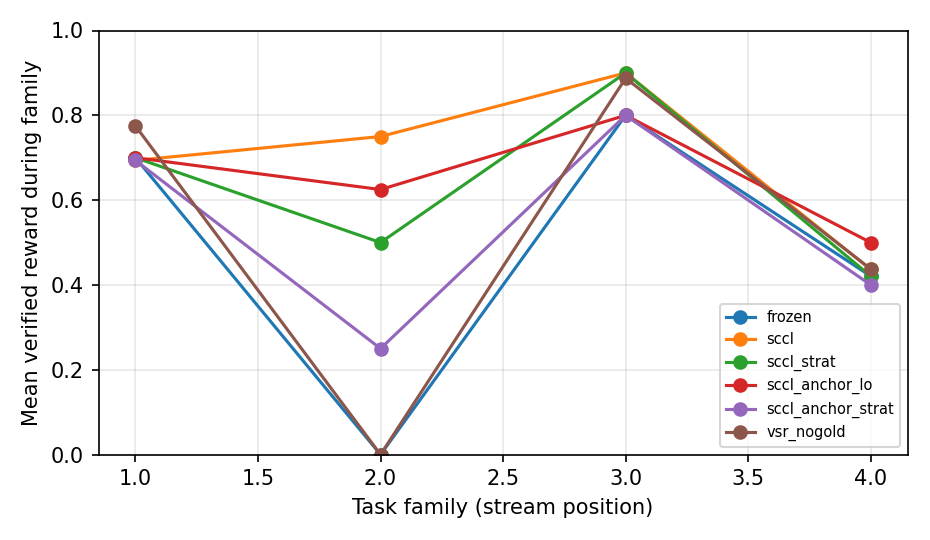
\includegraphics[width=\columnwidth]{fig_v5_family_curves.png}}{%
  \fbox{\parbox[c][3.2cm][c]{0.92\columnwidth}{\centering figure pending --- rendered from the completed run (runs/sccl\_v5\_fixed)}}}
\caption{Mean verified reward per family phase (stream order: arith, math\_word, string, drift) for the six corrected-factorial learners, seed 42. Rendered by \texttt{gcl/plots.py} from the run's measured trajectories; no hand-edited series.}
\label{fig:v5families}
\end{figure}

\begin{figure}[htbp]
\centering
\IfFileExists{fig_v5_frontier.png}{%
  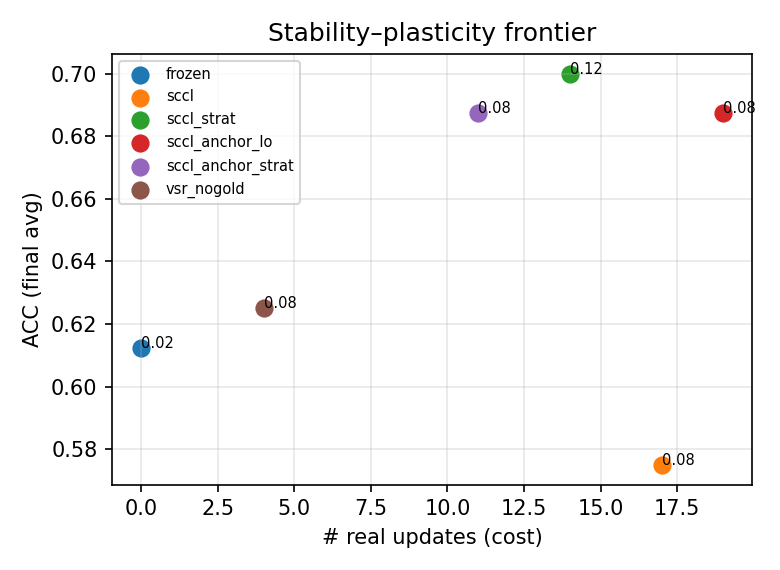
\includegraphics[width=0.86\columnwidth]{fig_v5_frontier.png}}{%
  \fbox{\parbox[c][3.2cm][c]{0.8\columnwidth}{\centering figure pending --- rendered from the completed run (runs/sccl\_v5\_fixed)}}}
\caption{Stability--plasticity frontier of the corrected factorial: final ACC against the number of real (accepted) updates; annotations give forgetting. The candidate composition is read against the \textsc{sccl} cell per the pre-registered rules.}
\label{fig:v5frontier}
\end{figure}

\textbf{Pre-registered reading.} Three rules, fixed before observing the engaged-anchor data: \textbf{H1 (coverage main effect)} --- stratified veto alone lifts the arithmetic holdout over \textsc{sccl} without costing more than $0.02$ frontier; \textbf{H2 (anchor main effect)} --- the engaged anchor lifts arithmetic over \textsc{sccl} at comparable accuracy; \textbf{BREAKTHROUGH (composition)} --- the both-cell reaches arithmetic $\geq 0.55$ (closing most of the gap to frozen's $0.600$) at frontier $\geq$ \textsc{sccl} $-0.02$, in which case multi-seed confirmation (seeds 43/44, same protocol as v3) precedes any headline claim. Verdict: \textbf{all three rules fail on their arithmetic endpoint}, and the failure pattern is itself the finding. H1: stratification \emph{halves} the arithmetic holdout ($0.400 \to 0.200$) despite the stratified pool guaranteeing every family permanent check-pool representation. H2: the engaged anchor leaves arithmetic exactly where \textsc{sccl} leaves it ($0.400$) while lifting math ($0.500 \to 0.750$), drift ($0.600 \to 0.800$), and the frontier ($+0.500 \to +0.613$, best in the ladder, with the fewest rollbacks and the lowest forgetting). BREAKTHROUGH: the composition reaches $0.400 < 0.55$ arithmetic; its frontier condition passes ($+0.613 \geq +0.480$), so the rule fails on the endpoint, not on cost.

\textbf{What the failures share: the gate checks instances, not capabilities.} Two independent measurements converge. First, the stratification harm: guaranteeing each family permanent instance-level representation in the check pool did not protect the earliest family --- it made erosion \emph{worse}, because updates that break arithmetic \emph{generalization} while preserving the memorized arithmetic instances now pass a pool that always contains those instances, whereas under the unstratified pool some of them were coincidentally vetoed for also breaking a recent skill. Second, measurement-only gold telemetry on the seed-44 stratified run: 11 of 14 accepted updates degraded the arithmetic gold probe even though every one of them passed the stored self-tests that the gate re-verifies. The gate's own artifacts and the gold telemetry agree on the diagnosis: accepted updates are retaining the stored instances while eroding the capability those instances were evidence for. The anchor, acting inside the update, preserves capability broadly (math, drift, forgetting, BWT all improve) and fully neutralizes the stratification harm to arithmetic ($0.200 \to 0.400$), but it cannot hold the first family at $0.600$ once later-phase training proceeds --- its quadratic pull is outrun on the family the stream abandons earliest. The two mechanisms are complementary exactly as designed, and their composition is the best cell in the ladder; the residual is located in the \emph{evidence} the veto consumes. The pre-registered response is to upgrade that evidence: alongside each certified skill, manufacture a held-out \emph{capability probe} --- a numeric or paraphrase variant of the spec with fresh self-tests, never trained on --- and extend the veto to re-check the newest probe of each family, so an update is admitted only if the capability, not just the instance, survives it (Sec.~\ref{sec:v5b}).

\subsection*{SCCL v5b: capability probes --- upgrading the veto's evidence}
\label{sec:v5b}

The v5 verdict localizes the residual to the evidence the veto consumes: stored instances survive updates that erode the capability they certified. v5b attacks exactly that. For every certified skill the method additionally manufactures one \emph{capability probe}: for arithmetic and math-word families a numeric variant of the spec certified by the same majority vote; for string and drift families a paraphrase variant with freshly derived self-tests (reusing the bidirectional cross-validation of Sec.~\ref{sec:v5}'s neighborhood machinery). Probes are committed to the vault under a distinct kind and are \emph{never trained on}; a bounded pool keeps only the newest probe per family. The RRV veto is extended with one stratum that, before admitting an update, regenerates the newest probe of each family from the current model and requires it to still pass its fresh self-tests (canonical-format numeric match for math domains; assert-line execution for code). The rule is unchanged --- any of $n$ samples passing counts as retained --- only the evidence is stronger. A pre-registered bounded-damage guard prevents a single noisy probe from stalling learning: if capability vetoes exceed half of a family phase's attempts, the gate arms a margin re-check (two extra regenerations) before vetoing. All switches default off; the frozen and \textsc{sccl} rows of the v5b ladder must bit-reproduce the v5 rows at the same seeds as the inertness and determinism check. The pre-registered success rule is unchanged in form: the capability-probe stratified cell must reach arithmetic $\geq 0.55$ at frontier $\geq$ \textsc{sccl} $-0.02$, with multi-seed confirmation preceding any headline claim. The pre-registered prediction: if instance-retention-with-capability-loss is the dominant failure, capability vetoes will fire \emph{inside} family phases and the arithmetic holdout will stabilize near the frozen $0.600$ at a measurable plasticity cost. Results (Table~\ref{tab:v5b}): the capability probes are the strongest aggregate mechanism in this study so far, and they still fail the arithmetic endpoint --- and the failure mode is itself the next finding. The stratified capability cell is the best learner in the ladder on every aggregate measure: accuracy $0.694$, above even the frozen baseline ($0.613$) --- genuine absolute learning, not merely damage limitation; best backward transfer ($+0.214$); frontier $+0.562$, second only to the frozen model's free $+0.588$; and a \emph{perfect} math-word holdout ($1.000$, up from $0.500$ under plain \textsc{sccl} --- the largest single-family gain any mechanism has produced), with drift restored to the frozen level ($0.800$). Engagement was total: $15/15$ probes committed, and every one of the $24$ post-certification gates re-checked the newest probe of each family; the frozen and \textsc{sccl} rows bit-reproduce the v5 rows at the same seeds. Yet arithmetic lands at $0.375$ under \emph{both} probe rows --- the identical endpoint from two very different gate regimes ($9$ vs $15$ accepted updates) --- so H1 fails on the arithmetic endpoint, H2 passes (stratification adds everything else: math $0.750 \to 1.000$, frontier $+0.494 \to +0.562$), and the breakthrough rule fails at $0.375 < 0.55$.

\begin{table}[t]
\centering
\small
\caption{SCCL v5b (seed 42). Capability probes compose into the best aggregate learner in the study (ACC $0.694$ beats the frozen baseline; math reaches $1.000$) while the first family's holdout remains unprotected at $0.375$ under both probe rows. Determinism check: frozen and \textsc{sccl} rows bit-identical to the v5 corrected factorial at the same seeds.}
\label{tab:v5b}
\begin{tabular}{lccccccccc}
\toprule
learner & ACC & BWT & Forget & Front. & Upd & arith & math & string & drift \\
\midrule
frozen              & 0.613 & +0.132 & 0.025 & +0.588 & 0  & 0.600 & 0.250 & 0.800 & 0.800 \\
\textsc{sccl}       & 0.575 & +0.095 & 0.075 & +0.500 & 17 & 0.400 & 0.500 & 0.800 & 0.600 \\
\textsc{sccl}\,+\,cap              & 0.625 & +0.145 & 0.131 & +0.494 & 9  & 0.375 & 0.750 & 0.600 & 0.775 \\
\textsc{sccl}\,+\,cap\,+\,strat    & 0.694 & +0.214 & 0.131 & +0.562 & 15 & 0.375 & 1.000 & 0.600 & 0.800 \\
\bottomrule
\end{tabular}
\end{table}

\textbf{Why the probe passes while capability erodes.} The arithmetic probe existed from the first family phase and was re-verified at every later gate; every accepted update passed it; the arithmetic holdout still fell from $0.600$ to $0.375$. A per-update gold telemetry pass (measurement only, never fed to any decision; \texttt{scripts/v5b\_telemetry.py}) localizes the damage precisely. In the best row, in-phase arithmetic/math training \emph{net-preserves} the arithmetic holdout (it returns to the frozen $0.600$ by the end of the math phase); the terminal damage is inflicted by \emph{cross-family} updates, and every one of them passed all live capability probes --- a $0\%$ true-positive rate on real arithmetic damage. The single largest blow is one drift-phase update (tuple manipulation) that drops the arithmetic holdout from $0.600$ to $0.150$ in a step while all three family probes return pass. The mechanism is that \emph{family is coarser than skill axis}: the arithmetic family is skill-heterogeneous (numeric/geometry tasks frozen at $1.0$ alongside list/tuple-manipulation tasks frozen at $0.2$), and the newest-per-family arithmetic probe is a word-reversal witness --- a string-manipulation axis. The catastrophic update destroys the unwitnessed numeric/geometry axis (one holdout task $1.0 \to 0.2$) while leaving the witnessed string axis intact. One held-out variant per family is therefore too thin a witness not merely within a spec but across a family's skill axes (the pre-registered branch-(c) diagnosis, now refined). A second, unanticipated mechanism compounds it: under high veto pressure the accepted updates are \emph{selected} to fit the current instance and the probe tightly --- the capability row's \emph{trained} arithmetic score rises to $0.800$ while its arithmetic holdout falls to $0.375$, a generalization gap of $0.425$ versus $0.200$ under plain \textsc{sccl}. The gate is a filter, not a regularizer: filtering reshapes the accepted-update distribution toward instance-narrow survivors and never pulls weights, and the string family pays the starvation cost ($0.800 \to 0.600$, forgetting $0.131$ vs $0.075$). Capability-level evidence is confirmed as the right direction --- it converted the v5 instance gap into the strongest aggregate result in the study --- but the witness must be both \emph{wider} (an ensemble spanning a family's skill axes, not $k$ variants of one spec) and paired with an in-update regularizer that protects the axes no probe witnesses.

\section{Discussion}
SCCL reframes the supervision problem of deployed continual learning: instead of asking ``who provides the tests?'', it asks ``when is the model's own executable interpretation of a spec trustworthy enough to learn from?'' Discriminative consensus gives a computable answer, the unanimous rule turns mastered skills into protected memory, and RRV converts that memory into a stability mechanism. The ladder shows each ablation doing its job: unsafe baselines collapse (verification matters), no-consensus degrades (cross-bag agreement matters) --- and full gold supervision underperforms gold-free certification. Gold is neither necessary for safe continual learning nor, when injected as reference targets, sufficient for it; the productive role left for gold is verifying the model's \emph{own} solutions (\textsc{vsr\_nogold}), which SCCL's self-tests largely reproduce for free --- on accuracy the gold-free match is within run-to-run variance, and the residual frontier gap is quantified above.

The v2/v3/v4 arc is a lesson about \emph{where} stability mechanisms can and cannot act. v1's gate protects trained points; v2 extends protection to a manufactured generalization neighborhood, and measurably buys stability with plasticity (more vetoes, fewer accepted updates, lower accuracy); v3 moves the same neighborhood evidence upstream of the gradient, where a rejection costs a certification attempt instead of a weight update --- and multi-seed, that admission filter raises accuracy and its stability but \emph{not} forgetting (Table~\ref{tab:v3}). The general lesson: gates decide \emph{which} updates happen; they cannot control what an accepted update does to weights the gate never inspects. Filtering fragile targets is strictly cheaper than vetoing them after training, and the gate remains the right backstop for distribution drift --- but unvisited general capability must be defended \emph{inside} the update itself, which is the role of v4's base anchor (Sec.~\ref{sec:v4}). The v4 ladder adds a methodological lesson to that arc. Its anchor, as first implemented, silently failed to engage --- a state-dict key mismatch left the penalty matching no parameter --- and the plausible mechanism story that run initially seemed to support (a weak anchor as a pure plasticity win) dissolved the moment its rows were compared against the seed-matched controls that had existed all along in the v3 seed ladder (Table~\ref{tab:v4}). We treat the retraction as part of the record: an audit trail that checks wiring but not effect can pass while a mechanism is inert, so every mechanism reported here now carries an \emph{engagement test} verifying the effect itself. The post-mortem attributes the arithmetic erosion to the gate's recency window: certified families leave the check pool when the stream moves on, so their erosion is never vetoed. In-update regularization and out-of-gradient coverage attack that residual by different routes and are complementary by construction, which is why v5 tests their composition in a factorial design rather than a fifth sequential variant (Sec.~\ref{sec:v5}).

A methodological point deserves emphasis. Continual-learning benchmarks for LLMs rarely report seed variance; ours, measured directly, exceeds most published-style mechanism deltas on this stream. We read this as a warning for the area and as a design constraint: mechanisms must either produce effects robust across seeds or be reported with them.

\textbf{Limitations.} Single 3B model, one GPU, one small stream; gold-agreement telemetry uses a small probe; correlated misinterpretation of ambiguous specs remains the fundamental failure mode of any gold-free method; open-decision admission under variant-generation failure is a necessary conservatism whose rate we log per run. Scaling the stream, model size, seed count, and probe is ongoing work.

\section{Related Work}
\textbf{Classical continual learning.} Stability mechanisms fall into three families. Regularization methods penalize movement of important parameters --- EWC uses a Fisher-based importance estimate \cite{kirkpatrick2017ewc}, Synaptic Intelligence accumulates an online path integral of gradient contributions \cite{si}, and MAS ties importance to output sensitivity \cite{mas}. Replay methods constrain the gradient against stored past examples, either episodically \cite{er} or through projected gradients over a memory buffer \cite{gem,agem}. Architecture-based methods partition or grow capacity per task. SCCL intersects both main families with a twist: its certified rehearsal is replay in which the buffer was curated without gold (every pair is consensus-certified), and v4's base anchor is a regularizer whose anchor point $\theta_0$ and importance weights carry no data-derived signal at all --- the target is the model's own initialization, so the penalty is gold-free by construction rather than by bookkeeping.

\textbf{Continual learning of LLMs.} Recent work documents and attacks forgetting under continual fine-tuning of large models \cite{luo2025forgetting,luo2023investigating}, including LoRA-based approaches that isolate tasks in orthogonal low-rank subspaces \cite{olora} or gate adapter integration \cite{gil}, benchmarks for the setting \cite{trace}, and surveys of the area \cite{shi2025survey}. These methods largely assume each task's supervision is available at training time; the deployment regime we study removes that assumption entirely --- no task labels, no gold tests, no gold holdout --- and asks whether stability can still be enforced. Empirically our setting reproduces the signature finding of the LLM-forgetting literature (capability loss concentrates in components the stream under-visits) but shows it arises \emph{inside accepted updates}, which accept/reject gating alone cannot prevent.

\textbf{Self-improvement without external verification.} Self-training lineages bootstrap from a model's own outputs: STaR iterates rationalization and fine-tuning \cite{zelikman2022star}, self-consistency decodes and votes over reasoning paths \cite{wang2022self}, self-repair and self-debug recondition on execution feedback \cite{chen2024teaching}, and self-improvement filters self-generated instruction data by model-scored preference \cite{selfimprove}. All of these retain an external filter --- task answers, an oracle, gold executables, or a preference model trained on labels --- and process supervision likewise trains verifiers from human annotations \cite{verify}. Execution-grounded rewards appear in program-synthesis RL, and safe deployment typically relies on holdout gates. SCCL is, to our knowledge, the first to replace \emph{both} the target-quality verifier and the safety gate with self-certified, structurally gold-free mechanisms, and to enforce that property with adversarial tests.

\begin{thebibliography}{99}
\bibitem{hu2021lora} E.~J. Hu et al., ``LoRA: Low-Rank Adaptation of Large Language Models,'' arXiv:2106.09685, 2021.
\bibitem{kirkpatrick2017ewc} J.~Kirkpatrick et al., ``Overcoming Catastrophic Forgetting in Neural Networks,'' \emph{PNAS} 114(13):3521--3526, 2017.
\bibitem{si} F.~Zenke, B.~Poole, and S.~Ganguli, ``Continual Learning Through Synaptic Intelligence,'' in \emph{Proc. ICML}, 2017.
\bibitem{mas} R.~Aljundi, F.~Babiloni, M.~Elhoseiny, M.~Rohrbach, and T.~Tuytelaars, ``Memory Aware Synapses: Learning What (not) to Forget,'' in \emph{Proc. ECCV}, 2018.
\bibitem{gem} D.~Lopez-Paz and M.~Ranzato, ``Gradient Episodic Memory for Continual Learning,'' in \emph{Advances in Neural Information Processing Systems (NIPS)}, 2017.
\bibitem{agem} A.~Chaudhry, M.~Ranzato, M.~Rohrbach, and M.~Elhoseiny, ``Efficient Lifelong Learning with A-GEM,'' in \emph{Proc. ICLR}, 2019.
\bibitem{er} D.~Rolnick, A.~Ahuja, J.~Schwarz, T.~Lillicrap, and G.~Wayne, ``Experience Replay for Continual Learning,'' in \emph{Advances in Neural Information Processing Systems (NeurIPS)}, 2019.
\bibitem{luo2025forgetting} Y.~Luo, Z.~Yang, F.~Meng, Y.~Li, J.~Zhou, and Y.~Zhang, ``An Empirical Study of Catastrophic Forgetting in Large Language Models During Continual Fine-tuning,'' \emph{IEEE/ACM Trans. Audio, Speech, and Language Processing} 33:3776--3786, 2025, arXiv:2308.08747.
\bibitem{luo2023investigating} Y.~Luo, Z.~Yang, X.~Bai, F.~Meng, J.~Zhou, and Y.~Zhang, ``Investigating Forgetting in Pre-Trained Representations Through Continual Learning,'' arXiv:2305.05968, 2023.
\bibitem{olora} X.~Wang, T.~Chen, Q.~Ge, H.~Xia, R.~Bao, R.~Zheng, Q.~Zhang, T.~Gui, and X.~Huang, ``Orthogonal Subspace Learning for Language Model Continual Learning,'' in \emph{Findings of EMNLP}, pp. 10658--10671, 2023.
\bibitem{gil} Y.-S.~Liang, J.-R.~Chen, and W.-J.~Li, ``Gated Integration of Low-Rank Adaptation for Continual Learning of Large Language Models,'' in \emph{Advances in Neural Information Processing Systems (NeurIPS)}, 2025.
\bibitem{trace} X.~Wang, Y.~Zhang, T.~Chen, S.~Gao, S.~Jin, X.~Yang, Z.~Xi, R.~Zheng, Y.~Zou, T.~Gui, Q.~Zhang, and X.~Huang, ``TRACE: A Comprehensive Benchmark for Continual Learning in Large Language Models,'' arXiv:2310.06762, 2023.
\bibitem{shi2025survey} H.~Shi, Z.~Xu, H.~Wang, W.~Qin, W.~Wang, Y.~Wang, Z.~Wang, S.~Ebrahimi, and H.~Wang, ``Continual Learning of Large Language Models: A Comprehensive Survey,'' \emph{ACM Computing Surveys} 58(5):1--42, 2025.
\bibitem{chen2023humaneval} M.~Chen et al., ``Evaluating Large Language Models Trained on Code,'' arXiv:2107.03374, 2021.
\bibitem{austin2021mbpp} J.~Austin, A.~Odena, M.~Nye, M.~Bosma, H.~Michalewski, D.~Dohan, E.~Jiang, C.~Cai, M.~Terry, Q.~Le, and C.~Sutton, ``Program Synthesis with Large Language Models,'' arXiv:2108.07732, 2021.
\bibitem{zelikman2022star} E.~Zelikman, Y.~Wu, J.~Mu, and N.~D. Goodman, ``STaR: Bootstrapping Reasoning With Reasoning,'' in \emph{Advances in Neural Information Processing Systems (NeurIPS)}, 2022.
\bibitem{wang2022self} X.~Wang et al., ``Self-Consistency Improves Chain of Thought Reasoning in Language Models,'' in \emph{Proc. ICLR}, 2023.
\bibitem{chen2024teaching} L.~Chen, M.~Rabe, E.~Austin, D.~Charlier, Y.~Minsky, and V.~Misra, ``Teaching Large Language Models to Self-Debug,'' in \emph{Proc. ICLR}, 2024.
\bibitem{selfimprove} J.~Huang, S.~S.~Gu, L.~Hou, Y.~Wu, X.~Wang, H.~Yu, and J.~Han, ``Large Language Models Can Self-Improve,'' in \emph{Proc. EMNLP}, pp. 1051--1068, 2023.
\bibitem{verify} H.~Lightman, V.~Kosaraju, Y.~Burda, H.~Edwards, B.~Baker, T.~Lee, J.~Leike, J.~Schulman, I.~Sutskever, and K.~Cobbe, ``Let's Verify Step by Step,'' in \emph{Proc. ICLR}, 2024, arXiv:2305.20050.
\end{thebibliography}

\section{Reproducibility}
\begin{lstlisting}[language=bash]
python -m gcl.runner --config configs/sccl_main.json
python -m gcl.report --run runs/sccl_main --out paper/results.tex
python -m gcl.runner --config configs/sccl_v2.json
python -m gcl.report --run runs/sccl_v2 --out paper/results_v2.tex --prefix vtwo
python -m gcl.runner --config configs/sccl_v3.json   # seeded (torch_seed=42)
python scripts/run_seeds.py --config configs/sccl_v3.json --seeds 42,43,44
python -m gcl.report --aggregate runs/sccl_v3_seeds --out paper/results_v3.tex --prefix vthree
python -m gcl.runner --config configs/sccl_v4.json   # v4 base-anchor ladder (seeded)
python -m gcl.runner --config configs/sccl_v5.json   # v5 anchor x coverage factorial (seeded)
python -m pytest tests/test_sccl.py   # gold-free proof suite
\end{lstlisting}
Gold-freeness is checked by 66 tests: AST audits of \texttt{selfcert.py} (covering the probe-manufacture and neighborhood-check APIs), signature inspection, certification semantics under real sandbox execution, poisoned-gold adversarial environments, bidirectional probe cross-validation, certified-rehearsal mixing, admission-time neighborhood certification (open/closed decision policy), RRV rollback behavior across skills, probes, and math entries, the v4 base anchor (per-learner wiring, ladder isolation, decision-independence, per-learner $\lambda$ override, config-vs-learner-registry consistency so ladder rows cannot be silently skipped, and --- added after the key-mismatch disclosure of Sec.~\ref{sec:results} --- two engine-level \emph{effect-engagement} tests: key-set agreement between the anchor snapshot and the penalty loop, and strictly reduced distance-to-init under anchoring), and the v5 family-stratified veto pool (deterministic per-family selection, $2\times2$ factorial wiring, and back-compat of the default recency path so every pre-v5 row stays bit-identical).

\end{document}
